%%%%%%%%%%%%%%%%%%%%%%%%%%%%%%%%%%%%%%%%%%%%%%%%%%%%%%%%%%%%%%%%%%%%%%%%%%%%%%%
% Uni Duesseldorf
% Lehrstuhl fuer Datenbanken and Informationssysteme
% Vorlage fuer Bachelor-/Masterarbeiten
% Optimiert fuer den Original-Latex-Kompiler LATEX.EXE (LaTeX=>PS=>PDF)
% Version 1.4 - 2.3.2010
%%%%%%%%%%%%%%%%%%%%%%%%%%%%%%%%%%%%%%%%%%%%%%%%%%%%%%%%%%%%%%%%%%%%%%%%%%%%%%%

%%%%%%%%%%%%%%%%%%%%%%%%%%%%%%%%%%%%%%%%%%%%%%%%%%%%%%%%%%%%%%%%%%%%%%%%%%%%%%%
%%%%%%%%%%% BEGINN EINSTELLUNG FUER DIE ARBEIT. UNBEDINGT ERFORDERLICH! %%%%%%%
%%%%%%%%%%%%%%%%%%%%%%%%%%%%%%%%%%%%%%%%%%%%%%%%%%%%%%%%%%%%%%%%%%%%%%%%%%%%%%%
% Geben Sie Ihren Namen hier an
\newcommand{\bearbeiter}{Alina Elterman}

% Geben Sie hier den Titel Ihrer Arbeit an
\newcommand{\titel}{Game-theoretic Analysis of Strategyproofness in Cake-cutting Protocols}

% Geben Sie das Datum des Beginns and Ende der Bachelorarbeit ein
\newcommand{\beginndatum}{05. September 2011}
\newcommand{\abgabedatum}{05.~Dezember~2011}

% Geben Sie die Namen des Erst- and Zweitgutachters an
\newcommand{\erstgutachter}{Prof. Dr.~J\"org Rothe}
\newcommand{\zweitgutachter}{Prof. Dr.~Peter Kern}

% Falls Sie die Arbeit zweiseitig ausdrucken wollen,
% benutzen Sie die folgende Zeile mit
% \AN fuer zweiseitigen Druck
% \AUS fuer einseitigen Druck
\newcommand{\zweiseitig}{\AUS}

% Falls die Arbeit in englischer Sprache verfasst 
% werden soll, dann benutzen Sie die folgende Zeile mit
% englisch fuer englische Sprache
% deutsch fuer deutsche Sprache
\newcommand{\sprache}{englisch}
%%%%%%%%%%%%%%%%%%%%%%%%%%%%%%%%%%%%%%%%%%%%%%%%%%%%%%%%%%%%%%%%%%%%%%%%%%%%%%%%%
%%%%%%%%%%%%%%%%%%%%%%%%%%%%%%% ENDE EINSTELLUNGEN %%%%%%%%%%%%%%%%%%%%%%%%%%%%%%
%%%%%%%%%%%%%%%%%%%%%%%%%%%%%%%%%%%%%%%%%%%%%%%%%%%%%%%%%%%%%%%%%%%%%%%%%%%%%%%%%

% Die folgende Zeile NICHT EDITIEREN oder loeschen
% (Zum Ab�ndern der BA-Vorlage in eine MA-Vorlage muessen sie
% jedoch die Datei titelmakros1.tex selbst editieren.)
%%%%%%%%%%%%%%%%%%%%%%%%%%%%%%%%%%%%%%%%%%%%%%%%%%%%%%%%%%%
% Obere Titelmakros. Editieren Sie diese Datei nur, wenn
% Sie sich ABSOLUT sicher sind, was Sie da tun!!!
% (Z.B. zum Abaendern der BA-Vorlage in eine MA-Vorlage)
% Uni Duesseldorf
% Lehrstuhl fuer Datenbanken und Informationssysteme
% Version 2.2 - 2.3.2010
%%%%%%%%%%%%%%%%%%%%%%%%%%%%%%%%%%%%%%%%%%%%%%%%%%%%%%%%%%%
\newcommand{\AN}{twoside}
\newcommand{\AUS}{}
%\newcommand{\englisch}{}
%\newcommand{\deutsch}{\usepackage[german]{babel}}

%% Die folgenden auskommentierten Optionen dienen der automatischen
%% Erkennung des Latex-Kompilers und dem Setzen der davon abh�ngigen
%% Einstellungen. Bei Problem z.B. mit dem Einbinden von verschiedenen
%% Grafiktypen bei Verwendung von PdfLatex oder Latex, einfach die
%% verschiedenen \usepackage(s) ausprobieren. (Mit diesen Einstellungen
%% funktionierte diese Vorlage bei der Verwenundg von latex.exe als
%% Kompiler bei den meisten Studierenden.)

%\newif\ifpdf \ifx\pdfoutput\undefined
%\pdffalse % we are not running pdflatex
%\else
%\pdfoutput=1 % we are running pdflatex
%\pdfcompresslevel=9 % compression level for text and image;
%\pdftrue \fi

\documentclass[11pt,a4paper, \zweiseitig]{article}



%\usepackage[iso]{umlaute}
\usepackage[latin1]{inputenc}
\usepackage{palatino} % palatino Schriftart
%\usepackage{makeidx} % um ein Index zu erstellen
\usepackage{tocbibind}
\usepackage[T1]{fontenc} %fuer richtige Trennung bei Umlauten
\usepackage{fancybox} % fuer die Rahmen
\usepackage{shortvrb}
\usepackage{ifthen}
\ifthenelse{\equal{\sprache}{deutsch}}{\usepackage[ngerman]{babel}}{}

\usepackage{lmodern} 
\usepackage{amsmath}
\usepackage{amssymb}
\usepackage{pdfpages}
\usepackage{hyperref}
%\usepackage{fancyheadings}
\usepackage{fancyhdr}
\usepackage{amsfonts}
\usepackage{amsthm}
\usepackage{color}
\usepackage{stmaryrd}
\usepackage{nomencl}
\usepackage[normalem]{ulem} 
\newcommand{\markup}[1]{\uline{#1}}
% Befehl umbenennen in abk
\let\abk\nomenclature

\usepackage{a4wide} % ganze A4 Weite verwenden

%\ifpdf
%\usepackage[pdftex,xdvi]{graphicx}
%\usepackage{thumbpdf} %thumbs fuer Pdf
%\usepackage[pdfstartview=FitV]{hyperref} %anklickbares Inhaltsverzeichnis
%\else
\usepackage[dvips,xdvi]{graphicx}
\usepackage{hyperref} %anklickbares Inhaltsverzeichnis
%\fi

%%%%%%%%%%%%%%%%%%%%%%% Massangaben fuer die Arbeit %%%%%%%%%%%%%%%
\setlength{\textwidth}{15cm}

\setlength{\oddsidemargin}{35mm}
\setlength{\evensidemargin}{25mm}

\addtolength{\oddsidemargin}{-1in}
\addtolength{\evensidemargin}{-1in}

%\makeindex
% Umgebungen f"ur S�tze usw.
\newtheorem*{bemerkung*}{Bemerkung}
\newtheorem*{defi}{Definition}
\newtheorem*{defi*}{Definition}
\newtheorem*{bezeichnungen}{Bezeichnungen}
\newtheorem*{fakt}{Fakt}
\newtheorem*{beispiel}{Beispiel}
\newtheorem*{bsp}{Beispiel}
\newtheorem*{beispiel*}{Beispiel}
\newtheorem*{satz}{Satz}
\newtheorem*{satz*}{Satz}
\newtheorem*{lem}{Lemma}
\newtheorem*{protokoll*}{Protokoll}
\newtheorem*{idee}{Idee}

%definition of new commands
\newcommand{\DGEF}{\text{\textbf{DGEF}}}

\begin{document}

%\setcounter{secnumdepth}{4} %Nummerieren bis in die 4. Ebene
%\setcounter{tocdepth}{4} %Inhaltsverzeichnis bis zur 4. Ebene

\pagestyle{headings}

\sloppy % LaTeX ist dann nicht so streng mit der Silbentrennung
\MakeShortVerb{\�}

\parindent0mm
\parskip0.5em


{
\textwidth170mm 
\oddsidemargin30mm 
\evensidemargin30mm 
\addtolength{\oddsidemargin}{-1in}
\addtolength{\evensidemargin}{-1in}

\parskip0pt plus2pt

% Die Raender muessen eventuell fuer jeden Drucker individuell eingestellt
% werden. Dazu sind die Werte fuer die Abstaende `\oben' und `\links' zu
% aendern, die von mir auf jeweils 0mm eingestellt wurden.

%\newlength{\links} \setlength{\links}{10mm}  % hier abzuaendern
%\addtolength{\oddsidemargin}{\links}
%\addtolength{\evensidemargin}{\links}

\begin{titlepage}
\vspace*{-1.5cm}
  \raisebox{17mm}{
    \begin{minipage}[t]{70mm}
      \begin{center}
        %\selectlanguage{german}
        {\Large INSTITUT F�R INFORMATIK\\}
        {\normalsize
          Lehrstuhl f�r Komplexit\"atstheorie und Kryptologie
\\
        }
        \vspace{3mm}
        {\small Universit�tsstr. 1 \hspace{5ex} D--40225 D�sseldorf\\}
     \end{center}
    \end{minipage}
  }
  \hfill
  
\includegraphics[width=130pt]{bilder/HHU_Logo}
  \vspace{14em}

% Titel
  \begin{center}
      	\baselineskip=55pt
    	\textbf{\huge \titel}
  	 	\baselineskip=0 pt
   \end{center}

  %\vspace{7em}

\vfill

% Autor
  \begin{center}
    \textbf{\Large
      \bearbeiter
    }
  \end{center}

  \vspace{35mm}
 
% Pr�fungsordnungs-Angaben
  \begin{center}
    %\selectlanguage{german}
    
%%%%%%%%%%%%%%%%%%%%%%%%%%%%%%%%%%%%%%%%%%%%%%%%%%%%%%%%%%%%%%%%%%%%%%%%%
% Ja, richtig, hier kann die BA-Vorlage zur MA-Vorlage gemacht werden...
%%%%%%%%%%%%%%%%%%%%%%%%%%%%%%%%%%%%%%%%%%%%%%%%%%%%%%%%%%%%%%%%%%%%%%%%%
    {\Large Bachelorarbeit}

    \vspace{2em}

    \begin{tabular}[t]{ll}
      Beginn der Arbeit:& \beginndatum \\
      Abgabe der Arbeit:& \abgabedatum \\
      Gutachter:         & \erstgutachter \\
                         & \zweitgutachter \\
    \end{tabular}
  \end{center}

\end{titlepage}

}

%%%%%%%%%%%%%%%%%%%%%%%%%%%%%%%%%%%%%%%%%%%%%%%%%%%%%%%%%%%%%%%%%%%%%
\clearpage
\begin{titlepage}
  ~                % eine leere Seite hinter dem Deckblatt
\end{titlepage}
%%%%%%%%%%%%%%%%%%%%%%%%%%%%%%%%%%%%%%%%%%%%%%%%%%%%%%%%%%%%%%%%%%%%%
\clearpage
\begin{titlepage}
\vspace*{\fill}

\section*{Erkl�rung}

%%%%%%%%%%%%%%%%%%%%%%%%%%%%%%%%%%%%%%%%%%%%%%%%%%%%%%%%%%%
% Und hier ebenfalls ggf. BA durch MA ersetzen...
%%%%%%%%%%%%%%%%%%%%%%%%%%%%%%%%%%%%%%%%%%%%%%%%%%%%%%%%%%%

Hiermit versichere ich, dass ich diese Bachelorarbeit
selbstst�ndig verfasst habe. Ich habe dazu keine anderen als die
angegebenen Quellen und Hilfsmittel verwendet.

\vspace{25 mm}

\begin{tabular}{lc}
D�sseldorf, den \abgabedatum \hspace*{2cm} & \underline{\hspace{6cm}}\\
& \bearbeiter
\end{tabular}

\vspace*{\fill}
\end{titlepage}

%%%%%%%%%%%%%%%%%%%%%%%%%%%%%%%%%%%%%%%%%%%%%%%%%%%%%%%%%%%%%%%%%%%%%
% Leerseite bei zweiseitigem Druck
%%%%%%%%%%%%%%%%%%%%%%%%%%%%%%%%%%%%%%%%%%%%%%%%%%%%%%%%%%%%%%%%%%%%%

\ifthenelse{\equal{\zweiseitig}{twoside}}{\clearpage\begin{titlepage}
~\end{titlepage}}{}

%%%%%%%%%%%%%%%%%%%%%%%%%%%%%%%%%%%%%%%%%%%%%%%%%%%%%%%%%%%%%%%%%%%%%
\clearpage
\begin{titlepage}

\section*{\ifthenelse{\equal{\sprache}{deutsch}}{Zusammenfassung}{Abstract}}


%%%%%%%%%%%%%%%%%%%%%%%%%%%%%%%%%%%%%%%%%%%%%%%%%%%%%%%%%%%%%%%%%%%%%%%%%%%%%%%%%
%%%%%%%%%%%%%%%%%%%%%%%%%%%% BEGINN ZUSAMMENFASSUNG %%%%%%%%%%%%%%%%%%%%%%%%%%%%%
%%%%%%%%%%%%%%%%%%%%%%%%%%%%%%%%%%%%%%%%%%%%%%%%%%%%%%%%%%%%%%%%%%%%%%%%%%%%%%%%%
\begin{comment}
\begin{enumerate}
\item What is the problem?
\item Why interesting?
\item How to solve?
\item What is the result?
\end{enumerate}
\end{comment}
%%%%%%%%%%%%%%%%%%%%%%%%%%%%%%%%%%%%%%%%%%%%%%%%%%%%%%%%%%%%%%%%%%%%%%%%%%%%%%%%%
%%%%%%%%%%%%%%%%%%%%%%%%%%%%% ENDE ZUSAMMENFASSUNG %%%%%%%%%%%%%%%%%%%%%%%%%%%%%%
%%%%%%%%%%%%%%%%%%%%%%%%%%%%%%%%%%%%%%%%%%%%%%%%%%%%%%%%%%%%%%%%%%%%%%%%%%%%%%%%%

% Die folgende Zeile NICHT EDITIEREN oder loeschen
%%%%%%%%%%%%%%%%%%%%%%%%%%%%%%%%%%%%%%%%%%%%%%%%
% Untere Titelmakros. Editieren Sie diese Datei nur, wenn Sie sich
% ABSOLUT sicher sind, was Sie da tun!!!
%%%%%%%%%%%%%%%%%%%%%%%%%%%%%%%%%%%%%%%%%%%%%%%
\vspace*{\fill}
\end{titlepage}

%%%%%%%%%%%%%%%%%%%%%%%%%%%%%%%%%%%%%%%%%%%%%%%%%%%%%%%%%%%%%%%%%%%%%
% Leerseite bei zweiseitigem Druck
%%%%%%%%%%%%%%%%%%%%%%%%%%%%%%%%%%%%%%%%%%%%%%%%%%%%%%%%%%%%%%%%%%%%%
\ifthenelse{\equal{\zweiseitig}{twoside}}
  {\clearpage\begin{titlepage}~\end{titlepage}}{}
%%%%%%%%%%%%%%%%%%%%%%%%%%%%%%%%%%%%%%%%%%%%%%%%%%%%%%%%%%%%%%%%%%%%%
\clearpage 
\tableofcontents
\thispagestyle{empty}
%\enlargethispage{\baselineskip}
\clearpage \setcounter{page}{1}
%%%%%%%%%%%%%%%%%%%%%%%%%%%%%%%%%%%%%%%%%%%%%%%%%%%%%%%%%%%%%%%%%%%%%
% Leere Seite, falls Inhaltsverzeichnis mit ungerader Seitenzahl und 
% doppelseitiger Druck
%%%%%%%%%%%%%%%%%%%%%%%%%%%%%%%%%%%%%%%%%%%%%%%%%%%%%%%%%%%%%%%%%%%%%
\ifthenelse{ \( \equal{\zweiseitig}{twoside} \and \not \isodd{\value{page}} \)}
	{\pagebreak \thispagestyle{empty} \cleardoublepage}{\clearpage}



%%%%%%%%%%%%%%%%%%%%%%%%%%%%%%%%%%%%%%%%%%%%%%%%%%%%%%%%%%%%%%%%%%%%%
%%%%%%%%%%%%%%%%%%%%%%%%% BEGINN TEXTTEIL %%%%%%%%%%%%%%%%%%%%%%%%%%%
%%%%%%%%%%%%%%%%%%%%%%%%%%%%%%%%%%%%%%%%%%%%%%%%%%%%%%%%%%%%%%%%%%%%%
\section{Introduction}
\begin{comment}
Erklären was ist FAIR DIVISION\\
%(kein sehr guter anfang gez. herr rothe)Strategic play, cheating, incentive compatible, risk aversion, truthfulness, strategyproof and a lot more. All of them are keywords of whether an algorithm can resist the actions of selfish players and their greediness.
Cake-cutting is part of interdisciplinary fields like economics, mathematics, operations research, political and computer science. Game theory is fulfilling the same property. Except for this fact, they have hardly something in common. While cake cutting is about fair division of a heterogeneous divisible good, where the studies are especially concentrated on types of fairness, game theory studies the strategies people use when making decisions.\\
The role of strategies has not been widely researched yet in the context of cake cutting. But their importance is indisputable, with respect to fairness. Imagine the following situation:
Example Cost Sharing from Algorithmic GT Noam Nissan chap. 15
\begin{itemize}
\item{division of sports tickets, health resources, computer networking resources, voting power, intellectual property licenses, costs for environmental improvements, etc}
\item{formalize fairness, including max-min fairness, proportional fairness, envy-free fairness, etc. which may or may not lead to stable allocations in the sense of say Nash Equilibrium, or strong Nash Equilibrium}
\end{itemize}
Es werden Auswirkungen von nicht ehrlichen Strategien auf die Gerechtigkeit von Protokollen betrachtet. Der approach der Neidfreiheit ist zu stark, da kein finite bounded Protokoll f"ur n >3 (>4 f"ur allgemein) bekannt ist. Dagegen w"are der approach der Proportionaltit"at zu schwach, $\dots$. Das notwendige Mittelmaß liefert der DGEF und so fällt der Focus dieser Arbeit auf die Möglichkeit den DGEF eines Protokolles durch unehrliche Strategien zu erhöhen. Die Analyse erfolgt mittels Spieltheorie.\\
\newline
$\cdot$ Able to show that the only strategy promising a fair share is the recommended one.
\end{comment}
\pagebreak
%%%%%%%%%%%%%%%%%%%%%%%%%%%%%%%%%%%%%%%%%%%%%%%%%%%%%%%%%%%%%%%%%%%%%%%%%%%%%%%%%%%%%%%%%%%%%%%%%%%%%%%%%%%%%%%%
%%%%%%%%%%%%%%%%%%%%%%%%%%%%%%%%%%%%%%%%%%%%%%%%%%%%%%%%%%%%%%%%%%%%%%%%%%%%%%%%%%%%%%%%%%%%%%%%%%%%%%%%%%%%%%%%
%%%%%%%%%%%%%%%%%%%%%%%%%%%%%%%%%%%%%%%%%%%%%%%%%%%%%%%%%%%%%%%%%%%%%%%%%%%%%%%%%%%%%%%%%%%%%%%%%%%%%%%%%%%%%%%%
\subsection{Related Work}
%In the field of cake-cutting the idea of counting envy- and envy-free-relations was introduced by Brams, Jones and Klamler (2007) mostly in the egalitarian way. It was edited to the utilitarian perspective and expanded by Lindner and Rothe (2009). The history and the scope of work done in other fields can be found in detail in the second work.\\
%\newline
\begin{comment}
\begin{tabular}{cll}
Truthfulness:&
$\cdot$ GT:&\\&
$\cdot$ MD:&\\&
$\cdot$ SC:&\\&
$\cdot$ CC(FD):&Ariel and Tamuz weakened the basic assumptions\\&&of cake-cutting and so only analysed special cases.\\&
$\cdot$ CC(MARA):&A lot of papers e.g. Lipton, Markakis $\dots$\\
\end{tabular}
\end{comment}
\pagebreak
%%%%%%%%%%%%%%%%%%%%%%%%%%%%%%%%%%%%%%%%%%%%%%%%%%%%%%%%%%%%%%%%%%%%%%%%%%%%%%%%%%%%%%%%%%%%%%%%%%%%%%%%%%%%%%%%
%%%%%%%%%%%%%%%%%%%%%%%%%%%%%%%%%%%%%%%%%%%%%%%%%%%%%%%%%%%%%%%%%%%%%%%%%%%%%%%%%%%%%%%%%%%%%%%%%%%%%%%%%%%%%%%%
%%%%%%%%%%%%%%%%%%%%%%%%%%%%%%%%%%%%%%%%%%%%%%%%%%%%%%%%%%%%%%%%%%%%%%%%%%%%%%%%%%%%%%%%%%%%%%%%%%%%%%%%%%%%%%%%
\section{Preliminaries}
\subsection{Preliminaries of Game Theory}
\begin{comment}
In this chapter, some basic concepts from game theory are described and directly applied to the cake-cutting problem. The comparison between the classes of games indicate that the best fitting game-theoretic model is the Bayesian game \cite{}. The development of this result and use of the associated solution concepts is described.
%Game theory can be seen as a tool for describing interaction in life's processes. The occurring problems can be simulated by games.  
%Non-cooperated game theory is about single selfish players, and in cooperated the main focus is on forming coalitions. For computer scientists especially the algorithmic game theory is of major interest, because $\dots$. 
\subsubsection{Concepts in Game Theory}
\begin{defi}{\textbf{(Game)}}\\
A \emph{non-cooperative (strategic) game} $\Gamma=(P_n,S,u)$ consists of the set of players $P_n$, the set of strategies $S$ and the set of utility functions (pay-off) of all players $u_i$.
\begin{itemize}
\item Each player in the set $P_n=\{p_1,\cdots,p_n\}$ behaves selfishly and rationally.
\item $\dots$
\end{itemize}
\end{defi}
Definition 2
(Outcome)
An outcome is any end-state of the system.



Definition 3 (Lottery-)
A lottery is a distribution over outcomes.

Definition 4 (Utility)
Utility is a real-valued quantity measuring an agent's happiness.

Definition 5 (Utility function)A utility function is a mapping from outcomes to utilities. The agent is indifferent between outcomes with equal utilities and strictly prefers outcomes with higher utilities.

Definition 6 (Rationality) A rational agent is an agent that acts to maximize its ex-
pected utility.

Definition 13 (Action profile) An action profile is a vector of actions, one per agent
in the system.

Definition 14 (Strategic equivalence) Two games are strategically equivalent if there
is a mapping between pure strategies in each game where for any strategy profile in
either game, there is a corresponding strategy profile in the other game that yields
exactly the same expected utility for every player.
Because of strategic equivalence, when analyzing games we frequently omit the
outcomes and map directly from action profiles to utilities:

Definition 15 (Game) A game is a system that has a set of agents, each of which has
a set of actions and a utility function over action profiles.

Definition 16 (Normal form game) A normal form game is a tabular representation
of a game. In the two-dimensional case (i.e. for two agents) the first agent chases the
row while the second choses the column. Each cell contains a vector of utility values,
one per player.

Definition 19 (Pure strategy (normal form game)) A pure strategy for a normal form
game is a single action.

Definition 20 (Mixed strategy) A mixed strategy is a probability distribution over
pure strategies.

Definition 21 (Support) The support of a. mixed strategy is the set of pure strategies
that have non-zero probability.
As with actions, it is useful to talk about agents' strategies in aggregate.

Definition 22 (Strategy profile) A strategy profile is a vector of strategies, one per
agent.
Unlike decision theory, there is not necessarily an optimal policy. Whether or not an
agent maximizes his utility by playing a particular strategy will depend on the behavior
of the other agents.

Definition 23 (Best response) A best response is a strategy (pure or mixed) which
maximizes the agent's expected utility given the strategies of all the other agents.

Definition 24 (Dominant strategy) A dominant strategy is a strategy that is a best
response regardless of the strategies of the other players.
A dominant strategy is strict if it is always strictly a best response, semi-strict if it
is sometimes a strict best response and weak otherwise.
With these concepts, we can finally define some "solution concepts" for normal
form games. These are stable configurations of the game.

Definition 25 (Nash equilibrium) A Nash Equilibrium is ct strategy profile where ev-
ery agent is playing a best response to the actions of the others.
We can characterize a Nash equilibrium as being a pure-strategy or mixed-strategy
equilibrium. It is also useful to distinguish equilibria in dominant strategies.

\begin{defi}{\textbf{(Pure/ Mixed Strategy)}}\\
A
\end{defi}

\begin{defi}{\textbf{(Strategies)}}\\
dominant, dominated, best response
\end{defi}


\begin{defi}{\textbf{(Nash-Equilibria)}}\\
A
\end{defi}

\subsubsection{Classes of Special Games}

\textbf{Information in Games}\\

\begin{defi}{\textbf{(Perfect/ Imperfect Information)}}\\
A
\end{defi}
Definition 33 (Perfect information extensive form game) Perfect information exten-
sive form games are games in tree representation where every inner node represents
a choice by a single agent, with the out-edges of the node being the possible actions.
Each leaf node is an outcome labeled by a vector of utilities (one per agent).

\begin{defi}{\textbf{(Complete/ Incomplete Information)}}\\
A
\end{defi}
Definition 35 (Imperfect information extensive form game) Imperfect information
extensive form games are extensive form games where the agent cannot distinguish
two or more choice nodes (those nodes are said to belong to an equivalence set).

%\textbf{Games with }\\

 Definition 37 (Pure strategy (extensive form game)) /\ pure strategy for an exten-
sive form game is a mapping from nodes or equivalence sets to actions {analogous
to a policy in decision theory.)
Definition 38 (Induced normal form (extensive form game)) We can convert an ex-
tensive form game into a normal form game (called the "induced normal form ") where
the normal form game's actions are pure strategies in the extensive form game. The
payoffs in the normal form game are taken front the leaf-node reached by following
those strategies.
Because every extensive form game has a corresponding induced normal form
game, it must have a Nash equilibrium (by Theorem 27).

\begin{defi}{\textbf{(Zero-Sum Game)}}\\
A 
\end{defi}
Cutting a cake is a non-zero-sum game since it allows players to get better off than $\nicefrac{1}{n}$-th. An exception is a homogeneous cake because the valuations over the cake are equal.\\
\newline
\begin{defi}{\textbf{(Repeated Game)}}\\
A 
\end{defi}

\begin{defi}{\textbf{(Bayesian Game)}}\\
A 
\end{defi}

Often, strategic interactions involve some notion of random events and private infor-
mation. We model these using Bayesian games. Many card games (for example, poker)
are instances of this type of interaction.
Definition 39 (Type) An agent's type is a complete representation of his private infor-
mation.
Definition 40 (Type profile) A type profile
is a vector of types, one per agent.
One simple but powerful way to represent Bayesian games is to say that the agents
have different information about which normal form game they are actually playing.
Definition (Bayesian Game)\\
A Bayesian Game is a set of players, each of which has a set of actions and a utility function mapping action and type profiles to utility. A Bayesian game also includes a distribution over type profiles.

Definition 43 (Pure strategy (Bayesian game)) A pure strategy in a Bayesian game
is a function mapping from type to action.
An alternative way of representing Bayesian games is to model them as extensive
form games where one of the agents is actually a random process (with all the real
agents having full common knowledge of the probabilities):
Definition 44 (Bayesian game (extensive form representation)) The extensive form
representation of a Bayesian game augments a conventional imperfect information ex-
tensive form game with "chance nodes" where each branch is chosen according to
some (commonly known) probability.
Extensive form representations of Bayesian games have the same pure strategy
space as regular extensive form games.
Definition 46 (Induced normal form (Bayesian game)) The induced normal form of
a Bayesian game is a normal form game where each action is a pure strategy in the
Bayesian game. The values in the cells of the table are filed in by computing the ex
ante expected utility of each pure strategy prof le.
When discussing the properties of Bayesian games, the amount of information
available must be defined (particularly when taking expectations). We characterize
this by the terms ex ante, ex interim and ex post.
Definition 47 (Ex ante) Ex ante refers to situations where no agent's type is fixed or
known.
Definition 48 (Ex interim) Ex interim refers to situations where exactly one agent's
type is known.
Definition 49 (Expost)
Ex ante refers to situations where all agent's types are known.\\
\newline
In many situations, players do not have complete information about their opponents. A seller of the house or a car may not know the valuation of potential buyers,
for example. These are situations of incomplete information. The approach to analyze these games is to convert the problem to one of imperfect information. In a game
of imperfect information, although a player may not know the type of another player,
every player in the game knows that it is a random realization from a known distribution. That is, a player’s type is thought of being chosen by the nature. Thus the
incomplete information about a player’s type is changed to the imperfect information
about the nature’s choice. A player’s type is only observed by the player himself. For
instance, although a seller may not know the valuation of a buyer on a car, but the
seller knows the buyer’s valuation is a random draw from the uniform distribution on
[$10,000, 15,000$]. A game of imperfect information is also called a Bayesian game.


\begin{defi}{\textbf{(Backwards Induction)}}\\
A 
\end{defi}
\begin{defi}{\textbf{(Subgame-perfect Equilibria)}}\\
A 
\end{defi}
A game can be represented in normal or in extended form. The normal form is advantageous for games where players move simultaneous, which is not often the case in cake-cutting. So the presentation in extended form as a game tree will be used in this work.
\end{comment}
\newpage
%%%%%%%%%%%%%%%%%%%%%%%%%%%%%%%%%%%%%%%%%%%%%%%%%%%%%%%%%%%%%%%%%%%%%%%%%%%%%%%%%%%%%%%%%%%%%%%%%%%%%%%%%%%%%%%%
%%%%%%%%%%%%%%%%%%%%%%%%%%%%%%%%%%%%%%%%%%%%%%%%%%%%%%%%%%%%%%%%%%%%%%%%%%%%%%%%%%%%%%%%%%%%%%%%%%%%%%%%%%%%%%%%
%%%%%%%%%%%%%%%%%%%%%%%%%%%%%%%%%%%%%%%%%%%%%%%%%%%%%%%%%%%%%%%%%%%%%%%%%%%%%%%%%%%%%%%%%%%%%%%%%%%%%%%%%%%%%%%%
\subsection{Preliminaries of Cake-cutting}
\subsubsection{Basics}
It is necessary to define the components and challenges of cake-cutting. But first, what exactly is cake-cutting about? It involves a set of $n \in \mathbb{N}$ players $P_n=\{p_1,\ldots,p_n\}$. It is assumed that each of them wants to get as much as possible of the divided resource. The goal is to find an allocation of a single, divisible and heterogeneous good between the $n$ players.\\ 
	\begin{figure}[h]
		\centering
 		 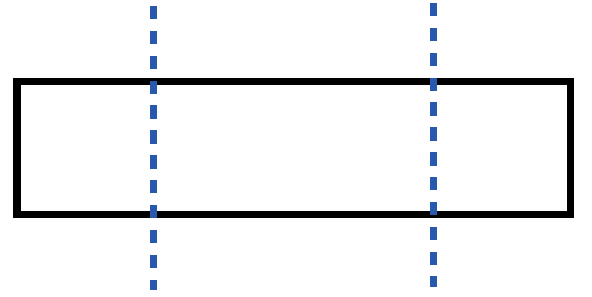
\includegraphics[width=120pt]{kek.pdf}
   \caption{Cake}Example for a visualisation of a cake with two cuts
  	 \end{figure} 
Such allocation has to be of a special kind, so that the involved players are pleased with the outcome. For the visualization it is common to use a rectangular cake. The division is performed by parallel cuts. The cake $X$ is represented by the unit interval $X=[0,1] \subseteq \mathbb{R}$. Each subinterval $X'\subseteq X$ or a sequence of disjoint subintervals $$\sideset{}{ }\bigcup\limits_{m\in\mathbb{N}}X'_m$$
with $X'_m\subseteq X$ is called a \emph{portion (or piece)}. The portion of the cake, which the player $p_i$ receives is denoted as $X_i$. The state is called an \emph{allocation}, when all portions of the cake are owned by players. Each piece has a public size, which can be computed as the sum of all border differences, and the private value of each player.\\

Every player $p_i\in P_n$ has a \emph{valuation function (valuation)} $v_i:\{X'|X' \subseteq X\} \rightarrow [0,1]$ with the following properties:
\begin{enumerate}
\item Non-negativity: $v_i(C)\geq 0$ for all $C\subseteq X.$
\item Normalisation: $v_i(\emptyset)=0$ and $v_i([0,1])=1.$
\item Additivity: $v_i(C \cup C')=v_i(C)+v_i(C')$ for disjoint
$C,C'\subseteq X.$\footnote{Monotonicity: If $C' \subseteq C$ then $v_i(C') \leq v_i(C)$. Monotonicity follows from additivity, because for the assumption $C' \subseteq C$ and $A:=C\backslash C'$: $v_i(C)=v_i(A\cup C')=v_i(A)+v_i(C')=\underbrace{v_i(C\backslash C')}_{\geq 0}+v_i(C')\geq v_i(C').$}
\item Divisibility: For all $C\subseteq [0,1]$ and all $\alpha \in
\mathbb{R}$, $0\leq \alpha \leq 1$, there exists a $B\subseteq C$, so that
$v_i(B)=\alpha \cdot v_i(C).$
\item  $v_i$ is continuous: If $0<x<y\leq 1$ with $v_i([0,x])=\alpha$ and
$v_i([0,y])=\beta$, then for every $\gamma \in [\alpha,\beta]$ there exists a $z \in [x,y]$ so that $v_i([0,z])=\gamma.$
\item Non-atomic:  $v_i([x,x])=0$ for all $x\in X.$
\end{enumerate}
After some basics it would be interesting to see how game-theory is applicable to cake-cutting. Example \ref{bsp1} illustrates the problem in a game-theoretic manner.
%
\begin{bsp}
\label{bsp1}
\textcolor{white}{x}\\\\
John Cocke and Tadao Kasami want to divide a chocolate-strawberry-cake. The cake is half chocolate from the left and the right part is strawberry. John Cocke got the first move and is thinking about making three different cuts. After the cuts the two pieces would have the following values:
	\begin{figure}[!h]
		\centering
 		 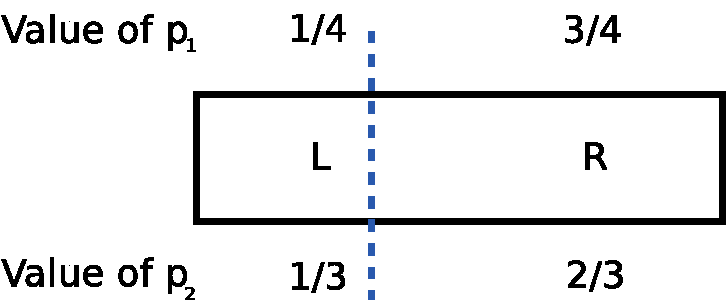
\includegraphics[width=390pt]{bilder/ex1.pdf}
   \caption{C$\&$K cake game}
  	 \end{figure}
  	 \newline
%%%%%%%%%%%%%%%%%%%%%%%%%%%%%%%%%%%%%%%%%%%%%%%%%%%%%%%%%%%%%%%%%%%%%%%%%%%%%%%%%%%%%%%%%%%%%%%%%%%%%%%%%%%%%%
\begin{table}[htb]
\centering
 \renewcommand{\arraystretch}{1.2} 
\begin{tabular}{c|c|c|c|}
\cline{2-4}
&\multicolumn{1}{|c|}{{Leftcut}}& {Middlecut}&{Rightcut}\\
\hline
\multicolumn{1}{|r|}{{L}}&$\left(\nicefrac{3}{4}, ?\right)$&$\left(\nicefrac{1}{2}, ?\right)$&$\left(\nicefrac{2}{5}, ?\right)$\\
\hline
\multicolumn{1}{|r|}{{R}}&$\left(\nicefrac{1}{4}, ?\right)$&$\left(\nicefrac{1}{2}, ?\right)$&$\left(\nicefrac{3}{5}, ?\right)$\\
\hline
\end{tabular}
\caption{C$\&$K cake game in normal form}\label{Table1}
\end{table}
Before doing so, he analyses his situation via the normal form:\\Since the valuation is a private function, he does not know the preferences of his colleague and has to assume that Tadao is indifferent between the two pieces. %By choosing not the middlecut he has the possibility to get more than a half, but also to make a loss.
Tadao is waiting for John's move and will choose his best strategy in the extended game form: 
%%%%%%%%%%%%%%%%%%%%%%%%%%%%%%%%%%%%%%%%%%%%%%%%%%%%%%%%%%%%%%%%%%%%%%%%%%%%%%%%%%%%%%%%%%%%%%%%%%%%%%%%%%%%%%
\begin{figure}[h!]
\begin{center}
	\begin{tikzpicture}
		\node[circle,draw,ball color=blue!10,shade=ball,inner sep=5pt] (n1) at (1,5) { };
		\node[circle,draw,ball color=blue!10,shade=ball,inner sep=5pt] (n2) at (5,3) {};
		\node[circle,draw,ball color=blue!10,shade=ball,inner sep=5pt] (n3) at (5,5) {};
		\node[circle,draw,ball color=blue!10,shade=ball,inner sep=5pt] (n4) at (5,7) {};
		\node[circle,draw,ball color=blue!10,shade=ball,inner sep=5pt] (n5) at (9,5.5) {};
		\node[circle,draw,ball color=blue!10,shade=ball,inner sep=5pt] (n6) at (9,4.5) {};
		\node[circle,draw,ball color=blue!10,shade=ball,inner sep=5pt] (n7) at (9,7.5) {};
		\node[circle,draw,ball color=blue!10,shade=ball,inner sep=5pt] (n8) at (9,6.5) {};
		\node[circle,draw,ball color=blue!10,shade=ball,inner sep=5pt] (n9) at (9,3.5) {};
		\node[circle,draw,ball color=blue!10,shade=ball,inner sep=5pt] (n10) at (9,2.5) {};

		\node[draw=none,fill=none] (t1) at (1,5.5) {1};
		\node[draw=none,fill=none] (t2) at (5,7.5) {2};
		\node[draw=none,fill=none] (t1) at (5,3.5) {2};
		\node[draw=none,fill=none] (t1) at (5,5.5) {2};

		\node[draw=none,fill=none,right] at (1.85,6.35) {Leftcut};
		\node[draw=none,fill=none,right] at (1.85,5.25) {Middlecut};
		\node[draw=none,fill=none,right] at (1.85,3.65) {Rightcut};
		\node[draw=none,fill=none,right] at (7,2.53) {R};
		\node[draw=none,fill=none,right] at (7,3.49) {L};
		\node[draw=none,fill=none,right] at (7,4.53) {R};
		\node[draw=none,fill=none,right] at (7,5.49) {L};
		\node[draw=none,fill=none,right] at (7,6.53) {R};
		\node[draw=none,fill=none,right] at (7,7.49) {L};
		\node[draw=none,fill=none,right] at (9.5,7.5) {$\left(\nicefrac{3}{4}, \nicefrac{1}{3}\right)$};
		\node[draw=none,fill=none,right] at (9.5,6.5) {$\left(\nicefrac{1}{4}, \nicefrac{2}{3}\right)$};
		\node[draw=none,fill=none,right] at (9.5,5.5) {$\left(\nicefrac{1}{2}, \nicefrac{3}{7}\right)$};
		\node[draw=none,fill=none,right] at (9.5,4.5) {$\left(\nicefrac{1}{2}, \nicefrac{4}{7}\right)$};
		\node[draw=none,fill=none,right] at (9.5,3.5) {$\left(\nicefrac{2}{5}, 1\right)$};
		\node[draw=none,fill=none,right] at (9.5,2.5) {$\left(\nicefrac{3}{5}, 0\right)$};
		
		
		\draw (n1) -- (n2);
		\draw (n1) -- (n3);
		\draw (n1) -- (n4);
		\draw (n3) -- (n5);
		\draw (n3) -- (n6);
		\draw (n4) -- (n7);
		\draw (n4) -- (n8);
		\draw (n2) -- (n9);
		\draw (n2) -- (n10);

	\end{tikzpicture}
	\caption{C$\&$K cake game in extended form}
\end{center}
\end{figure}
\newline For John the graph shows that if he stays secure he would obtain $v_1(X_1)=\nicefrac{1}{2}$. Otherwise he would get $\nicefrac{1}{4}$ or $\nicefrac{2}{5}$. So to make the middlecut is his best possible move.
\end{bsp}
%%%%%%%%%%%%%%%%%%%%%%%%%%%%%%%%%%%%%%%%%%%%%%%%%%%%%%%%%%%%%%%%%%%%%%%%%%%%%%%%%%%%%%%%%%%%%%%%%%%%%%%%%%%%%%%%
%%%%%%%%%%%%%%%%%%%%%%%%%%%%%%%%%%%%%%%%%%%%%%%%%%%%%%%%%%%%%%%%%%%%%%%%%%%%%%%%%%%%%%%%%%%%%%%%%%%%%%%%%%%%%%%%
%%%%%%%%%%%%%%%%%%%%%%%%%%%%%%%%%%%%%%%%%%%%%%%%%%%%%%%%%%%%%%%%%%%%%%%%%%%%%%%%%%%%%%%%%%%%%%%%%%%%%%%%%%%%%%%%
\subsubsection{Different Types of Fairness}
As indicated by the name, fairness plays an important role in fair division. But how is fairness defined? It can be seen as a valuation criterion of an allocation, which can be normalized and gives a possibility to compare different allocations. Usually the fairness criteria are distinguished between the following:
\begin{defi}{\textbf{(Proportional or Simple Fair)}}
\newline \emph{An allocation is \emph{proportional (simple fair)} if
$v_i(X_i) \geq 1/n$ for each player $p_i \in P_n$.}
\end{defi}
\begin{defi}{\textbf{(Envy-Freeness)}}
\newline \emph{An allocation is \emph{envy-free} if $v_i(X_i) \geq
v_i(X_j)$ for each couple of players $p_i, p_j \in P_n$.}
\end{defi}
\vsp
%\begin{defi}{\textbf{(Equity)}}
%\newline An allocation is \emph{equitable}, if $v_i(X_i) =
%\alpha$ for each player $p_i \in P_n$ and $0 \leq \alpha \leq 1$ \footnote{ If $\alpha = 1/n$ the allocation is called \emph{exact}.}.
%\end{defi}
%
%
The following theorem shows the correlation between the two allocations.
%
\begin{lem}
\textcolor{white}{x}
\begin{enumerate}
\item Every envy-free allocation is proportional.
\item An allocation between two players is envy-free if and only if it is proportional.
\end{enumerate}
\end{lem}
\begin{proof}
\textcolor{white}{x}
\begin{enumerate}
\item Proof by contradiction:\\ Assume $A$ is an envy-free allocation, but not proportional. From envy-freeness follows $v_i(X_i) \geq v_i(X_j)$ for each pair of players $p_i, p_j \in P_n$ and so each player has at least an as much valuable piece of cake as each other player. Hereby each player owns in his own valuation at least as much as $(n-1)$ other players and so at least $1/n$. \blitza The allocation $A$ is proportional. %$\lightning$ 
\\Therefore, all envy-free allocations are proportional.
\item ''$\Rightarrow$'' For two players an allocation is proportional if each player has at least the half of the cake in his valuation. So the first player thinks the second player got at most half of the cake in the valuation of the first player and vice versa. They would not envy each other.\\ ''$\Leftarrow$'' Follows from part 1.\\
\end{enumerate}
\end{proof}
A different criterion to valuate the quality of an allocation is efficiency. The correlation between the fairness criterion and efficiency can be found in \cite{eff}. 
\begin{defi}{\textbf{(Efficiency)}}
\newline \emph{An allocation \[A=\{X_1,\dots, X_n\}\] is \emph{efficient (Pareto optimal)} if there is no other allocation \[A'=\{X'_1,\dots, X'_n\}\] such that \[v_i(X_i)\leq v_i(X'_i)\] for all players $p_i \in P_n$ and for at least one player the inequality is strict.}
\end{defi}
%
\begin{lem}
\textcolor{white}{x}
	\begin{enumerate}
		\item Envy-freeness and proportionality does not imply efficiency.
		\item Efficiency does not ensure proportionality and so envy-freeness.
	\end{enumerate}
\end{lem}

\begin{proof}
\textcolor{white}{x}
	\begin{enumerate}
\item Imagine the following allocation with three players. Each player's portion consists up to three pieces. The value of the whole portion is (because of the additivity of the valuation) the sum of the pieces :
		\begin{table}[htb]
		\centering
		\renewcommand{\arraystretch}{1.2}
		\begin{tabular}{c|ccc}
		& $X_1 =X_1'\cup X_1''$& $X_2 =X_2'\cup X_2''$& $X_3 =X_3'\cup X_3''\cup X_3'''$\\
		\hline
		\multirow{2}*{$p_1$} & \multirow{2}*{\textcolor{blue}{$\nicefrac{1}{2}=\nicefrac{11}{12}+\nicefrac{1}{12}$}} & \multirow{2}*{$\nicefrac{1}{3}=0+\nicefrac{1}{3}$} & \multirow{2}*{$\nicefrac{1}{6}=0+\nicefrac{1}{12}+\nicefrac{1}{12}$}\\ \\
  \multirow{2}*{$p_2$} & \multirow{2}*{$\nicefrac{1}{3}=\nicefrac{1}{6}+\nicefrac{1}{6}$} & \multirow{2}*{\textcolor{blue}{$\nicefrac{1}{3}=\nicefrac{1}{3}+0$}} & \multirow{2}*{$\nicefrac{1}{3}=\nicefrac{1}{12}+\nicefrac{1}{12}+\nicefrac{1}{6}$}\\ \\
  \multirow{2}*{$p_3$} & \multirow{2}*{$0=0+0$} & \multirow{2}*{$\nicefrac{7}{18}=\nicefrac{6}{18}+\nicefrac{1}{18}$} & \multirow{2}*{\textcolor{blue}{$\nicefrac{11}{18}=\nicefrac{6}{18}+\nicefrac{3}{18}+\nicefrac{2}{18}$}}\\\\
 		\end{tabular}	 
\caption{Example for envy-freeness does not imply efficiency}\label{Table3}
\end{table}
\newline This allocation is obviously envy-free, since $v_i(X_i) \geq v_i(X_j)$ for all $i, j \in \{1,2,3\}, i \neq j$. It is not efficient, because if the players $p_1$ would get $p_2$'s portion $X_2''$, $p_1$ would get a more valuable piece of the cake and neither $p_2$ or $p_3$ would get less valuable pieces. Since in Theorem 1 was shown that envy-freeness implies proportionality, this example also demonstates that proportionality does not imply efficiency.
		\item Allocating the whole cake to one player is efficient, but definitely not proportional and therefore not envy-free.
	\end{enumerate}
\end{proof}
In \cite{brams2} the authors show a general argument that no finite bounded protocol can exist for such an allocation that is both proportional and efficient at the same time.
%%%%%%%%%%%%%%%%%%%%%%%%%%%%%%%%%%%%%%%%%%%%%%%%%%%%%%%%%%%%%%%%%%%%%%%%%%%%%%%%%%%%%%%%%%%%%%%%%%%%%%%%%%%%%%%%
%%%%%%%%%%%%%%%%%%%%%%%%%%%%%%%%%%%%%%%%%%%%%%%%%%%%%%%%%%%%%%%%%%%%%%%%%%%%%%%%%%%%%%%%%%%%%%%%%%%%%%%%%%%%%%%%
%%%%%%%%%%%%%%%%%%%%%%%%%%%%%%%%%%%%%%%%%%%%%%%%%%%%%%%%%%%%%%%%%%%%%%%%%%%%%%%%%%%%%%%%%%%%%%%%%%%%%%%%%%%%%%%%
\subsubsection{Different Types of Protocols}
It is very important to understand the types, structure and design of protocols, which are analysed in this paper.\\
\newline
Informal: (Algorithm)
\newline An \emph{algorithm} is an effective method for solving a problem, which is composed of a finite sequence of instructions.
\begin{defi}{\textbf{(Cake-Cutting-Protocol)}}
\newline \emph{A \emph{cake-cutting-protocol} (protocol for short) is an adaptive algorithm with a fixed number of players and the following properties:
\begin{itemize}
\item{A protocol consists of rules and strategies.\\ \emph{Rules} are requirements, which \emph{have to} be followed by the players without knowledge of their valuations and which execution can be verified.\\
\emph{Strategies} are recommendations, which \emph{can} be followed for getting the guaranteed fair share.}
\item Each player should be able to cut the cake at a specific moment independent of other players.
\item The protocol has no information about the valuation of the players, except of those it got from the steps before. It can not prove whether a player follows the strategy of the protocol.
\end{itemize}}
\end{defi}
\textbf{Comment:} Only such protocols are interesting where the actions of one player does not harm the other players. If a player does not follow his recommended strategy he may get less then a fair share.
\begin{defi}{\textbf{(Proportional/ Envy-Free Protocol)}}\\
\emph{A cake-cutting \emph{protocol} is called \emph{proportional} or \emph{envy-free} if independent by the players' valuations, each allocation is proportional or envy-free provided that all players follow the rules and strategies given by the protocol.}
\end{defi}
The development of such protocols is one of the main goals of cake-cutting \cite{bla}.

\begin{defi}{\textbf{(Finite (Discrete)/ Continuous (Moving-Knife) Protocol)}}
\newline \emph{A \emph{finite (discrete) protocol} gives a solution after a finite number of queries (valuations, marks, $\ldots$). In a \emph{continuous (a.k.a. moving-knife) protocol} a player has to make up to infinitely many queries.}
\end{defi}
\begin{defi}{\textbf{(Finite Bounded/ Finite Unbounded Protocol))}}
\newline \emph{A \emph{finite bounded protocol} has an upper bound of steps for all possible valuations. The number of those steps is only correlated, in some cases, with the number of players. A \emph{finite unbounded protocol} has no approximated number of steps.}
\end{defi}
The most desirable protocols are the finite bounded because of the ease of their implementation. \\
In the last sixty years the number of proportional finite bounded protocols have grown for an arbitrary number of players. But still no envy-free finite bounded protocol for an arbitrary $n$ is known \cite{chen:truth}. Only for three or less players a cake can be divided in a fixed number of steps, so that it is envy-free. For this reason only proportional protocols are considered in the further work.
%%%%%%%%%%%%%%%%%%%%%%%%%%%%%%%%%%%%%%%%%%%%%%%%%%%%%%%%%%%%%%%%%%%%%%%%%%%%%%%%%%%%%%%%%%%%%%%%%%%%%%%%%%%%%%%%
%%%%%%%%%%%%%%%%%%%%%%%%%%%%%%%%%%%%%%%%%%%%%%%%%%%%%%%%%%%%%%%%%%%%%%%%%%%%%%%%%%%%%%%%%%%%%%%%%%%%%%%%%%%%%%%%
%%%%%%%%%%%%%%%%%%%%%%%%%%%%%%%%%%%%%%%%%%%%%%%%%%%%%%%%%%%%%%%%%%%%%%%%%%%%%%%%%%%%%%%%%%%%%%%%%%%%%%%%%%%%%%%%
%\newpage
\section{Strategyproofness}
In practice, players are selfish and try to increase the value of their portion. In order to do so, they may for example report false valuations on parts of the cake. The goal is to prevent this.
\begin{defi}{\textbf{(Non-Truthful (Cheating) / Honest Player)}}\\
\emph{Every strategy is \emph{non-truthful} except of the strategy recommended by the protocol. A player who follows a non-truthful strategy will be called a \emph{non-truthful (cheating) player}. Otherwise the player is called \emph{honest}.}
\end{defi}
\begin{defi}{\textbf{(True Value Function)}}\\
\emph{A \emph{true value function} provides the value of the piece a player would receive by following the recommended strategy. This value is at least proportional in a proportional protocol.}
\end{defi}
A strategy is better than an other if the value of the obtained piece is bigger than in the other strategy.
\begin{defi}{\textbf{(Risk Aversion\cite{brams})}}\\
\emph{A player is \emph{risk averse} if he or she will never choose a strategy that may yield a more valuable piece of cake if it entails the possibility of getting less than a piece of a guaranteed size.}
\end{defi}
\begin{defi}{\textbf{(Strategyproofness of a Proportional Protocol\cite{lindner:degrees})}}\\
\emph{A proportional cake-cutting protocol is said to be \emph{strategyproof for risk averse players} (SPP for short) if a cheating player is no longer guaranteed a proportional share, whereas all other players (provided they play truthful) are still guaranteed to receive their proportional share.}
\end{defi}
%\textbf{Notice:} The actions of a player do not harm any of the other players.
%\begin{defi}{\textbf{(Truthful Allocation)}}
%An allocation is \emph{truthful} if the value of the cake obtained by a player by reporting false is not greater than by reporting the truth.
%\end{defi}

\begin{defi}{\textbf{(Strategyproofness in the sense of \cite{pie})}}\\
\emph{A protocol is \emph{strategyproof} if no player has a strategy that is assuredly better than his true value function.}
\end{defi}
The strategyproofness in the sense of \cite{pie} will be called weak strategyproofness (WSP for short) since it is always true for a proportional protocol (compare \cite{ccc}).
\begin{bsp}
\label{bsp222}
\textcolor{white}{x}\\\\
Assume the case when all valuations over the cake are equal, and all players, except of the cheating one follow the strategy provided by the protocol. Each of the honest player will get his proportional share, which the cheating player also values as $\nicefrac{1}{n}$ or more. Sharing a cake with $(n-1)$ other players means for the cheater that $\nicefrac{(n-1)}{n}$ or a more valuable part of the cake is allocated to other players and so only the value of $\nicefrac{1}{n}$ or less remains for him independent of his strategy. 
\end{bsp}
This characteristic is not significant, since valuations like in Example \ref{bsp222} of the players where the cheater would never get more than a proportional piece exist always.\\
A controversial point is that with this definition a player with a non-truthful strategy which obtains in one special case the same valuable piece, like the true value function and in all other strictly more valuable pieces would stay honest.\\
\newline
A stronger condition comes from the social choice literature:

\begin{defi}{\textbf{(Strategyproofness in the sense of \cite{why})}}\\
\emph{A protocol is \emph{strategyproof} if the true value function dominates every other strategy.}
\end{defi}

%Assume the statement is true, where each player acts truthful by following his best strategy, which yields to a maximum possible allocation for a player ''$\Leftrightarrow$'' Nash-equilibrium. But there is a problem, like \cite{malik} detected no known algorithm can fulfill this promise. The appealing alternative is the guarantee of a fair share for telling the truth.\\
In order to prevent misunderstandings, in this paper strategyproofness in the sense of \cite{why} will be called strong strategyproofness (SSP for short). It can be shown that none of the known cake-cutting protocols is able to fulfill the strong strategyproofness criteria, if the valuation of the players is not equal. All protocols shown in Chapter 3 work for two players in exactly the same way as cut $\&$ choose. Example \ref{bsp3} is similar to the one in \cite{chen:truth}.

\begin{bsp}
\label{bsp3}
\textcolor{white}{x}\\\\
John Warner Backus and Peter Naur are celebrating and Donald E. Knuth has brought a huge marzipan cake with an enormous cherry on the left side. John loves cherries and hates marzipan, and Peter is just very hungry. The pioneers of computer science apply cut $\&$ choose. Peter is the cutter, and his best strategy would be to separate the cake from the cherry. If Peter would have full knowledge (which would not violate the preconditions of strategyproofness in \cite{why}) about the valuations of John, he would always benefit from lying. From table \ref{Table4} he would know, that John would always take the left piece and so he could easily maximize the value of his portion. Hence, this algorithm is not strongly strategyproof.  
\end{bsp}
\begin{table}[htb]
\centering
 \renewcommand{\arraystretch}{1.2} 
\begin{tabular}{c|c|c|}
\cline{2-3}
&\multicolumn{1}{|c|}{{Only Cherry}}& {Middlecut}\\
\hline
\multicolumn{1}{|r|}{{L}}&$\left(\nicefrac{9}{10}, 1\right)$&$\left(\nicefrac{1}{2}, 1\right)$\\
\hline
\multicolumn{1}{|r|}{{R}}&$\left(\nicefrac{1}{10}, 0\right)$&$\left(\nicefrac{1}{2}, 0\right)$\\
\hline
\end{tabular}
\caption{B$\&$N cake game in normal form}\label{Table4}
\end{table}
In strong strategyproofness a player would never get a more valuable piece by lying independent of the valuation of the other players.\\
\newline
After a counterexample in \cite{ccc} the definition of strategyproofness in \cite{pie} was restricted to the case with non-equal valuations and for the general case changed to:

\begin{defi}{\textbf{(Strategyproofness in the sense of \cite{note})}}\\
\emph{A protocol is \emph{strategyproof} (SP for short) if no player has a strategy that is sometimes better or is at least as well as his true value function.}
\end{defi}
%The question arises whether a protocol can enforce truthfulness.\\
%An example will be the following case where $n$ players cut the cake in pieces with $v_i(X_i)=\nicefrac{1}{n}$ and then allocate them randomly to the players.\\
Imagine the situation where different sharing processes are happening more than once, and the player is interested in becoming best off in a long term view. A game-theoretical approach leads to the following definition:
\begin{defi}{\textbf{(Game-Theoretic Strategyproofness)}}\\
\emph{A protocol is \emph{game-theoretic strategyproof} (GTSP for short) if no player has a strategy with a higher expected value than the expected value of his true value function.}
\end{defi}

From results with the expected value it is difficult to conclude something about the other strategyproofness criterion. But it is possible to give a definition of strategyproofness with respect to game-theoretic strategyproofness and which can be compared to the other strategyproofness criterion.
\begin{defi}{\textbf{(Game-Theoretic Cake-Cutting Strategyproofness)}}\\
\emph{A protocol is \emph{game-theoretic cake-cutting strategyproof} (GTCCSP for short) if no player has a strategy that is better in at least one allocation than his true value function and in the other allocations at least as well as his true value function.}
\end{defi}

In Theorem \ref{thm5} the correlation between the above mentioned definitions of strategyproofness in cake-cutting is shown.

\begin{lem}
\label{thm5} The relation between different strategyproofness criteria is the following $$SPP \Rightarrow^{1} SP \Rightarrow^{2} GTCCSP \Rightarrow^{3} WSP$$ and
$$GTSP \Rightarrow^{4} GTCCSP.$$
%If the criteria is not fulfilled then $$notWPP \Rightarrow^{5} notGTCCSP \Rightarrow^{6} notSP \Rightarrow^{7} notSPP$$ and
%$$notGTCCSP \Rightarrow^{8} notGTSP$$
\end{lem}
\begin{proof}
\textcolor{white}{x}
\begin{enumerate}
\item If a protocol is $SPP$, then for every player in each strategy except of the recommended one exists at least one allocation $A_c$. In $A_c$ the cheating player $p_c$ receives a piece $X_c$ which is not proportional. Since in a proportional protocol all allocations guarantee a proportional share to every player, the value of his piece $X_c$ is less than he would obtain by following the recommended strategy. So the protocol is $SP$.   
%Es gibt keine Strategie mit alle Fälle mindestens proportional(Bei jeder strategie gibt es einen Fall mit weniger als proportional) \\
\item If a protocol is $SP$, then for every player in each strategy except of the recommended one exists at least one allocation $A_c$. In $A_c$ the cheating player $p_c$ receives a piece $X_{c}$ instead of $X_{\neg c}$, which he had received by following the recommended strategy. The value of $X_c$ is smaller than the value of $X_{\neg c}$. So no non-truthful strategy exist where the cheating player gets in all allocations at least the same valuable piece as in the recommended one. The protocol is $GTCCSP$.
%SP-Es gibt keine Strategie mit alle Fälle mindestens mehr als TRUE(prop oder mehr)(Bei jeder strategie gibt es einen Fall mit weniger als TRUE(prop oder mehr))\\
\item If a protocol is $GTCCSP$, then for every player in each strategy except of the recommended one exists at least one allocation $A_c$. In $A_c$ the cheating player $p_c$ receives a piece $X_{c}$ instead of $X_{\neg c}$, which he had received by following the recommended strategy. The value of $X_c$ is smaller or equal to the value of $X_{\neg c}$. So no non-truthful strategy exist where the cheating player gets in all allocations a more valuable piece than in the recommended one. The protocol is $WSP$.
%GTCCSP-Es gibt keine Strategie mit alle Fälle mindestens einmal mehr und keinmal weniger als TRUE(proportional oder mehr)(Bei jeder strategie gibt es einen Fall mit weniger oder keinen mit mehr als TRUE(proportional oder meh))\\
\item \textbf{Proof by contradiction:}\\
\newline
Assumption: If a protocol is $notGTCCSP$ then it is $GTSP$.\\
If a protocol is $notGTCCSP$, then there is one player with a strategy, which is not the recommended one. And for all allocations $A_{S_c}$ the cheating player $p_c$ receives a piece $X_{S_c}$ instead of $X_{S_{\neg c}}$, which he had received by following the recommended strategy. The value of $X_{S_c}$ is at least equal to the value of $X_{S_{\neg c}}$. In one allocation $A_{S'_c}$ the value of $X_{S'_c}$ is bigger than the value of $X_{S'_{\neg c}}$. Let $r$ be the number of all possible allocations. The expected value of the strategy ${S_c}$ al least equal with the expected value of the recommended strategy for the $r-1$ allocations since the value of the received pieces $X_{S_c}$ are at least equal to the value of the pieces $X_{S_{\neg c}}$. The expected value for the piece $X_{S'_c}$ is bigger than the expected value for $X_{S'_{\neg c}}$. \\
The general expected value is $E(S_c)\:\:$>$\:\:E(S_{\neg c})$ and is particularly not $E(S_c)\leq E(S_{\neg c})$ and the protocol is not $GTSP$. \blitza 
\newline
\newline
So $notGTCCSP \Rightarrow notGTSP$ and especially $GTSP \Rightarrow GTCCSP$.
%WSP-Es gibt keine Strategie mit alle Fälle mindestens mehr oder gleich TRUE(proportional oder mehr)(Bei jeder strategie gibt es einen Fall mit weniger oder gleich TRUE(proportional  oder mehr))\\
\end{enumerate}
\end{proof}
There are two independent types of strategyproofness to show for having a complete quantity of results. The start will be from the left side until one of the criteria is fulfilled, then the other strategyproofness further on the right follow from theorem 3. Independently a proof for the game-theoretic strategyproofness has to be given, since it cannot be followed from the other.  
\begin{lem} The relation between different strategyproofness criteria is the following $$SPP \not\Leftarrow^{1} SP \not\Leftarrow^{2} GTCCSP \not\Leftarrow^{3} WSP$$ and
$$GTSP \not\Leftarrow^{4} GTCCSP.$$
\end{lem}
\begin{proof}
\textcolor{white}{x}\\
\newline
Assume a protocol with two players $p_1$ and $p_2$ and two possible allocations $A_1$ and $A_2$, which have the same probability. In the recommended strategy $S_\neg c$ and in the non-truthful strategy $S_c$ the player $p_2$ gets the same values in $A_1$ and $A_2$. The values of $p_1$ are shown in the four tables below:\\
\begin{table}[htb]
		\centering
		\renewcommand{\arraystretch}{1.2}
		\begin{tabular}{cc}
		\begin{tabular}{c|cc}
		& in $A_1$& in $A_2$\\
		\hline
		$p_1(X_1)$ by $S_\neg c$ & {$\nicefrac{1}{2}$} & $\nicefrac{2}{3}$\\ 
  $p_1(X_1)$ by $S_c$& $\nicefrac{1}{2}$ & {$\nicefrac{1}{2}$}\\ 
 		\end{tabular}&
 				\begin{tabular}{c|cc}
		& in $A_1$& in $A_2$\\
		\hline
		$p_1(X_1)$ by $S_\neg c$ & {$\nicefrac{7}{8}$} & $\nicefrac{3}{4}$\\ 
  $p_1(X_1)$ by $S_c$& $\nicefrac{7}{8}$ & {$\nicefrac{3}{4}$}\\ 
 		\end{tabular}	 \\	
 		&\\ 
Case 1: $SPP \not\Leftarrow SP$ & Case 2: $SP \not\Leftarrow GTCCSP$\\
\begin{tabular}{c|cc}
		& in $A_1$& in $A_2$\\
		\hline
		$p_1(X_1)$ by $S_\neg c$ & {$\nicefrac{7}{8}$} & $\nicefrac{3}{4}$\\ 
  $p_1(X_1)$ by $S_c$& $1$ & {$\nicefrac{3}{4}$}\\ 
 		\end{tabular}&\begin{tabular}{c|cc}
		& in $A_1$& in $A_2$\\
		\hline
		$p_1(X_1)$ by $S_\neg c$ & {$\nicefrac{1}{2}$} & $\nicefrac{4}{7}$\\ 
  $p_1(X_1)$ by $S_c$& $1$ & {$\nicefrac{3}{7}$}\\ 
 		\end{tabular}\\	 
 		&\\
Case 3: $WSP \not\Leftarrow GTSP$& Case 4: $GTSP \not\Leftarrow GTCCSP$
\end{tabular}
\caption{Counter-examples for the correlation between the strategyproofness criteria}\label{234}
\end{table}
\newpage
\begin{enumerate}
\item[1] $SPP \not\Leftarrow SP$\\
In the strategy $S_c$ the player $p_1$ gets $p_1(X_1)=\nicefrac{1}{2}$. Since $\nicefrac{1}{2} < \nicefrac{2}{3}$ in $A_2$ the player $p_1$ would stay honest and this protocol is $SP$. But $1/2$ is proportional so the protocol is $notSPP$. 
\item[2] $SP \not\Leftarrow GTCCSP$\\Since $\nicefrac{7}{8} = \nicefrac{7}{8}$ in $A_1$ and $\nicefrac{3}{4} = \nicefrac{3}{4}$ in $A_2$ the player $p_1$ would stay honest and this protocol is $SP$. But no value in the non-truthful strategy is smaller than in the recommended strategy, so the protocol is $notSP$.
\item[3] $GTCCSP \not\Leftarrow WSP$\\
Since $\nicefrac{3}{4} = \nicefrac{3}{4}$ in $A_2$ and so the player $p_1$ has not a more valuable piece, he would stay honest and this protocol is $WSP$. But $1 > \nicefrac{7}{8}$ in $A_1$ and $\nicefrac{3}{4} = \nicefrac{3}{4}$ and the player $p_1$ has a more valuable piece in one allocation and the same value in the other so the protocol is $notGTCCSP$.
\item[4] $GTSP \not\Leftarrow GTCCSP$\\
Since $\nicefrac{3}{7} < \nicefrac{4}{7}$ in $A_2$ the player $p_1$ would stay honest and this protocol is $GTCCSP$. But the expected value for the recommended strategy is $\nicefrac{(\nicefrac{1}{2}+\nicefrac{4}{7})}{2}=\nicefrac{15}{28}$, which is smaller than $\nicefrac{(1+\nicefrac{3}{7})}{2}=\nicefrac{20}{28}$. So the protocol is $notGTSP$. 
\end{enumerate}
\end{proof}


\begin{bsp}
(Representation is inspired by \cite{Barbanel})
\begin{table}[htb]
\begin{tabular*}{\textwidth}[]{|@{\extracolsep{\fill}}l|l|c|}
\hline
\hline
\multicolumn{3}{|c|}{\textbf{Cut $\&$ choose for $n=2$}}\\
\hline
\multicolumn{1}{|c|}{\textbf{Rules}}& \textbf{Player $p_1$ strategy}& \multicolumn{1}{c|}{\textbf{Player $p_2$ strategy}}\\
\hline
$\:$1. Player $p_1$ partitions the cake $X$ &Partition $X$ into two&\\
$\:\:\:\:\:\:\:$into two pieces $\{X',X-X'\}$&pieces of equal value&\\
\hline
$\:$2. Player $p_2$ chooses one piece&&Choose the bigger value\\
\hline
$\:$3. Player $p_1$ gets the remaining&&\\
$\:\:\:\:\:\:\:$piece&&\\
\hline
\end{tabular*}
\caption{Cut $\&$ choose rules and strategies}\label{cc}
\end{table}
\end{bsp}
\begin{lem}
\label{thm6}
Cut $\&$ choose is strategyproof for proportional protocols.
\end{lem}
\begin{proof}
\textcolor{white}{x}\\\\
For the proof a general presentation of cut $\&$ choose game in extended form is used. W. l. o. g. the non-truthful cut is performed on the right part of the cake. The variables have the following restrictions: $$0 \leq a \leq 1,\: 0 < \epsilon \leq \nicefrac{1}{2},\: 0 \leq \delta \leq 1\tiny{-}a$$
\newpage
\begin{figure}[h!]
\begin{center}
	\begin{tikzpicture}
		\node[circle,draw,ball color=red!20,shade=ball,inner sep=5pt] (n1) at (1,5) { };
		\node[circle,draw,ball color=blue!10,shade=ball,inner sep=5pt] (n2) at (5,7) {};
		\node[circle,draw,ball color=red!20,shade=ball,inner sep=5pt] (n3) at (5,3) {};
		\node[circle,draw,ball color=blue!10,shade=ball,inner sep=5pt] (n4) at (9,8) {};
		\node[circle,draw,ball color=blue!10,shade=ball,inner sep=5pt] (n5) at (9,6) {};
		\node[circle,draw,ball color=blue!10,shade=ball,inner sep=5pt] (n6) at (9,4) {};
		\node[circle,draw,ball color=red!20,shade=ball,inner sep=5pt] (n7) at (9,2) {};

		\node[draw=none,fill=none] (t1) at (1,5.5) {1};
		\node[draw=none,fill=none] (t2) at (5,7.5) {2};
		\node[draw=none,fill=none] (t1) at (5,3.5) {2};

		\node[draw=none,fill=none,right] at (1.85,6.32) {Cut $\nicefrac{1}{2}$};		
		\node[draw=none,fill=none,right] at (1.85,3.55) {Cut $\neq \nicefrac{1}{2}$};
		\node[draw=none,fill=none,right] at (7,2.23) {R};
		\node[draw=none,fill=none,right] at (7,3.78) {L};
		\node[draw=none,fill=none,right] at (7,6.23) {R};
		\node[draw=none,fill=none,right] at (7,7.78) {L};
		\node[draw=none,fill=none,right] at (9.5,8) {$\left(\nicefrac{1}{2}, a\right)$};
		\node[draw=none,fill=none,right] at (9.5,6) {$\left(\nicefrac{1}{2}, 1 - a\right)$};
		\node[draw=none,fill=none,right] at (9.5,4) {$\left(\nicefrac{1}{2} + \epsilon, a + \delta \right)$};
		\node[draw=none,fill=none,right] at (9.5,2) {$\left(\color{red}{\nicefrac{1}{2} - \epsilon}\color{black}{}, 1 - a - \delta \right)$};

		\draw (n1) -- (n2);
		\draw (n1) -- (n3);
		\draw (n2) -- (n4);
		\draw (n2) -- (n5);
		\draw (n3) -- (n6);
		\draw (n3) -- (n7);

	\end{tikzpicture}
	\caption{Cut $\&$ choose game in extended form}
\end{center} 
\end{figure}
The red path is the general case, where by not following the recommended strategy player $p_1$ always becomes less than a proportional share. If Player $p_2$ would not choose the recommended strategy, he has to take a piece smaller than his proportional share. Both players would stay honest. Thus cut $\&$ choose is strategyproof for proportional protocols.
\end{proof}

\begin{lem}
\label{thm7}
Cut $\&$ choose is game-theoretic cake-cutting strategyproof.
\end{lem}
\begin{proof}
\textcolor{white}{x}\\\\
\textbf{Options for not following the recommended strategy:}
\begin{itemize}
\item Player $p_2$ takes the smaller piece. This can not be his intention, because then he has a piece with less value.
\item Player $p_1$ cuts the cake into two unequal pieces. The chance to get less in his valuation is equal to the chance to get more in his valuation of the cake. In stochastic terms it means, that the expected value at the end of the allocation will be in the honest case: $$ \nicefrac{1}{2} \cdot \nicefrac{1}{2}+\nicefrac{1}{2} \cdot \nicefrac{1}{2}=\nicefrac{1}{2} $$ and in the dishonest case: $$ \nicefrac{1}{2} \cdot X' +\nicefrac{1}{2} \cdot (X-X') =\nicefrac{1}{2} \cdot \underbrace{X}_{=1}=\nicefrac{1}{2}$$ According to the definition of game-theoretical strategyproofness in the case with equal expected values the player would stay honest. Cut $\&$ choose is game-theoretical strategyproof.
\end{itemize}
\end{proof}
\begin{bezeichnungen}
According to theorem \ref{thm5}, theorem \ref{thm6} and theorem \ref{thm7} cut $\&$ choose is\\strategyproof for proportional protocols, strategyproof, game-theoretical strategyproof, game-theoretical cake-cutting strategyproof and weak strategyproof.
\end{bezeichnungen}
%%%%%%%%%%%%%%%%%%%%%%%%%%%%%%%%%%%%%%%%%%%%%%%%%%%%%%%%%%%%%%%%%%%%%%%%%%%%%%%%%%%%%%%%%%%%%%%%%%%%%%%%%%%%%%%%
%%%%%%%%%%%%%%%%%%%%%%%%%%%%%%%%%%%%%%%%%%%%%%%%%%%%%%%%%%%%%%%%%%%%%%%%%%%%%%%%%%%%%%%%%%%%%%%%%%%%%%%%%%%%%%%%
%%%%%%%%%%%%%%%%%%%%%%%%%%%%%%%%%%%%%%%%%%%%%%%%%%%%%%%%%%%%%%%%%%%%%%%%%%%%%%%%%%%%%%%%%%%%%%%%%%%%%%%%%%%%%%%%
\section{Strategyproof Proportional Protocols}
The goal in this chapter is to analyse the strategyproofness of well-known protocols. First of all, they are rewritten into game-theoretic manner. Since each player has a truthful and a non-truthful strategy, a protocol with $n$ active players has at least $2n$ strategies. If the obtained value is not equal in different non-truthful strategies they have to be separated. So the amount of strategies would grow and would make the analysis very tediously.\\Luckily a protocol consists of a lot of repeats and actually each of the well-known protocols can be simplified to an interaction between two kinds of players. So the analysis of the whole game is unnecessary.\\
The proceed is as follows, the interactions between two kinds of players are represented in tables. A separation between rules and strategies is given. Afterwards the different strategies of a protocol are represented as an extended form game and the different kinds of strategyproofness are analysed.\\
An important pre-comment: Proportionality means each player gets $v_j(X_j)=\nicefrac{1}{n}$ for $1\leq j\leq n$. So if one player $p_n$ leaves the game with $v_i(X_n)<\nicefrac{1}{n}$ for $1\leq i\leq (n-1)$ it still holds for the next round that the cake $X=X-X_n$ is normalized and a proportional piece is $\nicefrac{1}{n-1}$ and not $\nicefrac{1+\epsilon_i}{n}$.
\\The complete protocols in the standard description as well as the proofs of their proportionality can be found in \cite{robertson:cake-cutting}.
%TODO: $\cdot$ Whether it is possible to get less envy-relations trough non truthful playing?
\subsection{The Steinhaus-Kuhn Lone Divider Protocol}
\begin{table}[htb]
\begin{tabular*}{\textwidth}{|@{\extracolsep{\fill}}l|c|r|}
\hline
\hline
\multicolumn{3}{|c|}{\textbf{Steinhaus-Kuhn Lone Divider protocol for arbitrary $n$}}\\
\hline
\multicolumn{1}{|c|}{\textbf{Rules}}& \textbf{Player $p_{1}$ strategy}&\multicolumn{1}{c|}{\textbf{Players in  $P_{n-1}$ strategy}}\\
\hline
$\:$1. Player $p_1$ cuts the cake $X$&Cut $X$ into $n$&\\
$\:\:\:\:\:\:\:$into $n$ pieces $\{X_1,\ldots,X_n\}$&pieces of equal value&\\
\hline
$\:$2. Players in $P_{n-1}$ mark $s$&&Mark $X_j$ if $v_i(X_j) \geq \nicefrac{1}{n}$\\$\:\:\:\:\:\:\:$pieces with $1 \leq s\leq n$&& for $1 \leq j \leq n$ and $2 \leq i \leq n$\\
\hline
$\:$3. If an allocation is impossible:&&\\$\:\:\:\:\:\:$Form the non-marked pieces&&\\$\:\:\:\:\:\:$to a new cake and exchange&&\\
$\:\:\:\:\:\:\:$the cutter (last cutter leaves&&\\$\:\:\:\:\:\:\:$with a non-marked piece)&&\\
\hline
\end{tabular*}
\caption{Lone divider rules and strategies}\label{ld}
\end{table}	 
\begin{figure}[h!]
\begin{center}
	\begin{tikzpicture}
		\node[circle,draw,ball color=red!20,shade=ball,inner sep=5pt] (n1) at (1,4) { };
		\node[circle,draw,ball color=red!20,shade=ball,inner sep=5pt] (n2) at (5,6) {};
		\node[circle,draw,ball color=red!20,shade=ball,inner sep=5pt] (n3) at (5,2) {};
		\node[circle,draw,ball color=blue!10,shade=ball,inner sep=5pt] (n4) at (5,7) {};
		\node[circle,draw,ball color=red!20,shade=ball,inner sep=5pt] (n5) at (5,1) {};
		\node[circle,draw,ball color=blue!10,shade=ball,inner sep=5pt] (n6) at (9,8) {};
		\node[circle,draw,ball color=blue!10,shade=ball,inner sep=5pt] (n7) at (9,7.6) {};
		\node[circle,draw,ball color=blue!10,shade=ball,inner sep=5pt] (n8) at (9,7.2) {};
		\node[circle,draw,ball color=blue!10,shade=ball,inner sep=5pt] (n9) at (9,6.8) {};
		\node[circle,draw,ball color=blue!10,shade=ball,inner sep=5pt] (n10) at (9,6.4) {};
		\node[circle,draw,ball color=blue!10,shade=ball,inner sep=5pt] (n11) at (9,6.0) {};
		\node[circle,draw,ball color=red!20,shade=ball,inner sep=5pt] (n20) at (9,2) {};
		\node[circle,draw,ball color=red!20,shade=ball,inner sep=5pt] (n18) at (9,1.6) {};
		\node[circle,draw,ball color=red!20,shade=ball,inner sep=5pt] (n19) at (9,1.2) {};
		\node[circle,draw,ball color=red!20,shade=ball,inner sep=5pt] (n17) at (9,0.8) {};
		\node[circle,draw,ball color=red!20,shade=ball,inner sep=5pt] (n16) at (9,0.4) {};
		\node[circle,draw,ball color=red!20,shade=ball,inner sep=5pt] (n15) at (9,0) {};
		
		\node[draw=none,fill=none] (t1) at (1,4.5) {1};
		\node[draw=none,fill=none] (t2) at (5,7.5) {$i$};
		\node[draw=none,fill=none] (t1) at (5,6.5) {$i$};
		\node[draw=none,fill=none] (t1) at (5,1.5) {$i$};
		\node[draw=none,fill=none] (t1) at (5,2.5) {$i$};

		\node[draw=none,fill=none,right] at (13.5,8.8) {Player in};
		\node[draw=none,fill=none,right] at (13.2,8.4) {$P_{n-1}$ strategy};
		\node[draw=none,fill=none,right] at (1.85,5.75) {All $\nicefrac{1}{n}$};
		\node[draw=none,fill=none,right] at (1.85,1.95) {All $\neq \nicefrac{1}{n}$};
		\node[draw=none,fill=none,right] at (2.99,3.05) {$n-1$ pieces $\neq \nicefrac{1}{n}$};
		\node[draw=none,fill=none,right] at (2.99,4.90) {$2$ pieces $\neq \nicefrac{1}{n}$};
		\node[draw=none,fill=none,right] at (13.5,8) {mark $\geq \nicefrac{1}{n}$};
		\node[draw=none,fill=none,right] at (13.5,7.6) {mark $= \nicefrac{1}{n}$};
		\node[draw=none,fill=none,right] at (13.5,7.2) {mark none};
		\node[draw=none,fill=none,right] at (13.5,6.8) {mark $< \nicefrac{1}{n}$};
		\node[draw=none,fill=none,right] at (13.5,6.40) {mark all};
		\node[draw=none,fill=none,right] at (13.5,6) {mark $> \nicefrac{1}{n}$};
		\node[draw=none,fill=none,right] at (13.5,2) {mark $\geq \nicefrac{1}{n}$};
		\node[draw=none,fill=none,right] at (13.5,1.6) {mark $= \nicefrac{1}{n}$};		
		\node[draw=none,fill=none,right] at (13.5,1.2) {mark none};
		\node[draw=none,fill=none,right] at (13.5,0.8) {mark $< \nicefrac{1}{n}$};
		\node[draw=none,fill=none,right] at (13.5,0.40) {mark all};
		\node[draw=none,fill=none,right] at (13.5,0) {mark $> \nicefrac{1}{n}$};
		\node[draw=none,fill=none,right] at (4.75,4.1) {\Huge{.}};
		\node[draw=none,fill=none,right] at (4.75,3.9) {\Huge{.}};
		\node[draw=none,fill=none,right] at (4.75,3.7) {\Huge{.}};
		\node[draw=none,fill=none,right] at (2.75,4.1) {\Huge{.}};
		\node[draw=none,fill=none,right] at (2.75,3.7) {\Huge{.}};
		\node[draw=none,fill=none,right] at (2.75,3.9) {\Huge{.}};
		\node[draw=none,fill=none,right] at (5.5,2) {\huge{...}};
		\node[draw=none,fill=none,right] at (5.5,6) {\huge{...}};
		\node[draw=none,fill=none,right] at (9.5,8) {$\left(\nicefrac{1}{n}, \nicefrac{1+\delta_1}{n}\right)$};
		\node[draw=none,fill=none,right] at (9.5,7.6) {$\left(\nicefrac{1}{n}, \nicefrac{1}{n}\right)$\blitza};
		\node[draw=none,fill=none,right] at (9.5,7.2) {$\left(\nicefrac{1}{n}, \nicefrac{(1-\delta_2)}{n}\right)$\blitza};
		\node[draw=none,fill=none,right] at (9.5,6.8) {$\left(\nicefrac{1}{n}, \nicefrac{(1-\delta_3)}{n}\right)$\blitza};
		\node[draw=none,fill=none,right] at (9.5,6.4) {$\left(\nicefrac{1}{n}, \nicefrac{(1-\delta_4)}{n}\right)$\blitza};
		\node[draw=none,fill=none,right] at (9.5,6.0) {$\left(\nicefrac{1}{n}, \nicefrac{(1+\delta_5)}{n}\right)$};
		\node[draw=none,fill=none,right] at (9.5,2) {$\left(\color{red}{}\nicefrac{(1\pm\epsilon_1)}{n}\color{black}{}, \nicefrac{1+\delta_{5n-4}}{n}\right)$};
		\node[draw=none,fill=none,right] at (9.5,1.6) {$\left(\color{red}{}\nicefrac{(1\pm\epsilon_2)}{n}\color{black}{}, \nicefrac{1}{n}\right)$\blitza};
		\node[draw=none,fill=none,right] at (9.5,1.2) {$\left(\color{red}{}\nicefrac{(1\pm\epsilon_3)}{n}\color{black}{}, \nicefrac{(1-\delta_{5n-3})}{n}\right)$\blitza};
		\node[draw=none,fill=none,right] at (9.5,0.8) {$\left(\color{red}{}\nicefrac{(1\pm\epsilon_4)}{n}\color{black}{}, \nicefrac{(1-\delta_{5n-2})}{n}\right)$\blitza};
		\node[draw=none,fill=none,right] at (9.5,0.4) {$\left(\color{red}{}\nicefrac{(1\pm\epsilon_5)}{n}\color{black}{},\nicefrac{(1+\delta_{5n-1})}{n}\right)$\blitza};
		\node[draw=none,fill=none,right] at (9.5,0.0) {$\left(\color{red}{}\nicefrac{(1\pm\epsilon_5)}{n}\color{black}{},\nicefrac{(1+\delta_{5n})}{n}\right)$};
		
		
		\draw (n1) -- (n2);
		\draw (n1) -- (n3);
		\draw (n1) -- (n4);
		\draw (n1) -- (n5);
		\draw (n4) -- (n6);
		\draw (n4) -- (n7);
		\draw (n4) -- (n8);
		\draw (n4) -- (n9);
		\draw (n4) -- (n10);
		\draw (n4) -- (n11);
		\draw (n5) -- (n15);
		\draw (n5) -- (n20);
		\draw (n5) -- (n19);
		\draw (n5) -- (n18);
		\draw (n5) -- (n17);
		\draw (n5) -- (n16);

	\end{tikzpicture}
	\caption{Lone divider cake game in extended form}
\end{center}

\end{figure}
\begin{lem}
Lone divider protocol is not game-theoretic cake-cutting strategyproof.
\end{lem}
\pagebreak
\begin{proof}
\textcolor{white}{x}\\\\
For showing that lone divider is $notGTCCSP$ it is necessary to have at least one cheating player $p_c$. This player has a non-truthful strategy with $v_c(X_c)>v_c(X_t)$ in one allocation and $v_c(X_c) \geq v_c(X_t)$ for all other allocations. The proof is divided in two parts. In the first part the case $v_c(X_c)>v_c(X_t)$ can be is illustrated with an example. And in the second part a case distinction shows that this player is never getting a less valuable piece.
The non-truthful strategy is to mark $X_j$ if $v_c(X_j) > \nicefrac{1}{n}$ for $1 \leq j \leq n$, or in the only case when all pieces have the same value to mark all of them.\\
\newline
\textbf{Part I: Example for a successful non-truthful strategy}\\
\newline
Imagine the following allocation with three players. The player $p_1$ is going to cheat.
		\begin{table}[htb]
		\centering
		\renewcommand{\arraystretch}{1.2}
		\begin{tabular}{c|ccc}
		& $X_L$& $X_M$& $X_R$\\
		\hline
		$p_3$ (divider)  & $\nicefrac{1}{3}$ & {$\nicefrac{1}{3}$} & $\nicefrac{1}{3}$ \\
  $p_2$ (rank 2) & {$\nicefrac{3}{5}$} & $\nicefrac{2}{5}$ & $0$\\
  $p_1$ (rank 1)& {$\nicefrac{1}{2}$} & $\nicefrac{1}{3}$ & $\nicefrac{1}{6}$
 		\end{tabular}
 		
\caption{Example for a successful non-truthful strategy}\label{Table10}
\end{table}

		\begin{table}[htb]
		\centering
		\renewcommand{\arraystretch}{1.2}
		\begin{tabular}{cc}
		\multicolumn{2}{c}{The acceptable pieces}\\
		By following the recommended strategy:& By following the non-truthful strategy:\\
 		\begin{tabular}{c|ccc}
		& $X_L$& $X_M$& $X_R$\\
		\hline
		$p_3$ (divider)  &  \Checkmark &  \Checkmark &  \Checkmark \\
  $p_2$ (rank 2) &  \Checkmark & \Checkmark &  \XSolidBrush \\
  $p_1$ (rank 1)&  \Checkmark &  \Checkmark & \XSolidBrush
 		\end{tabular}&
 		\begin{tabular}{c|ccc}
		& $X_L$& $X_M$& $X_R$\\
		\hline
		$p_3$ (divider)  &  \Checkmark &  \Checkmark &  \Checkmark \\
  $p_2$ (rank 2) &  \Checkmark & \Checkmark &  \XSolidBrush \\
  $p_1$ (rank 1)&  \Checkmark & \XSolidBrush & \XSolidBrush
 		\end{tabular}
 		\end{tabular}
 		
\caption{Acceptable pieces by a successful non-truthful strategy}\label{Table11}
\end{table}
\newpage An allocation is possible since each pieces is acceptable for at least one different player.\\ \newline If player $p_1$ chooses the recommended strategy $S_\neg c$:\\
There are no players with just one acceptable piece, so the player with the highest rank can choose first.
Player $p_2$ chooses $X_L$ and player $p_1$ gets $X_M$ with $p_1(X_M)= \nicefrac{1}{3}$. The divider gets the last piece.\\
\newline
If player $p_1$ chooses the non-truthful strategy $S_c$:\\
There is one players with just one acceptable piece, so this player chooses first.
Player $p_1$ chooses $X_L$ with $p_1(X_L)= \nicefrac{1}{2}$ and player $p_2$ gets $X_M$. The divider gets the last piece.\\
The value of players $p_1$ piece in the non-truthful strategy $S_c$ is $p_1(X_L)=\nicefrac{1}{2}>\nicefrac{1}{2}=p_1(X_M)$ than in the recommended strategy $S_\neg c$. So the player $p_1$ is at least in one allocation better off with the non-truthful strategy than in the recommended one.\\
\newline
\textbf{Part II: Case distinction for a successful non-truthful strategy} 
\begin{itemize}
\item[Case] 1: 
\item[Case] 2:
\item[Case] 3:
\item[Case] 4:
\item[Case] 5:
\item[Case] 6:
\end{itemize}
\end{proof}
\newpage
%%%%%%%%%%%%%%%%%%%%%%%%%%%%%%%%%%%%%%%%%%%%%%%%%%%%%%%%%%%%%%%%%%%%%%%%%%%%%%%%%%%%%%%%%%%%%%%%%%%%%%%%%%%%%%%%
%%%%%%%%%%%%%%%%%%%%%%%%%%%%%%%%%%%%%%%%%%%%%%%%%%%%%%%%%%%%%%%%%%%%%%%%%%%%%%%%%%%%%%%%%%%%%%%%%%%%%%%%%%%%%%%%
%%%%%%%%%%%%%%%%%%%%%%%%%%%%%%%%%%%%%%%%%%%%%%%%%%%%%%%%%%%%%%%%%%%%%%%%%%%%%%%%%%%%%%%%%%%%%%%%%%%%%%%%%%%%%%%%
\subsection{The Banach-Knaster Last-Diminisher Protocol}
The last diminisher protocol consists of $(n-2)$ rounds.\\The players are separated into two groups. In the first group is the player $p_i$ (with $i$ number of the round) and in the second group $P_{i+k}$ are all other players $p_j$ with $i <j\leq n$, $1\leq k \leq n-1$.\\ At the end of each round one player gets a piece and leaves the game. If it is player $p_i$ then player $p_{i+1}$ takes his place, otherwise player $p_i$ is player $p_{i+1}$ in the next round $i+1$ and players in group $P_{i+k}$ will be consecutively numbered. In the last round the two remaining players apply cut $\&$ choose. 

%\begin{lem}
% The Last-Diminisher-protocol has a $\DGEF$ of $\nicefrac{n(n-1)}{2}+2$.
%\end{lem}
\begin{table}[htb]
\begin{tabular*}{\textwidth}[]{|@{\extracolsep{\fill}}l|c|r|}
\hline
\hline
\multicolumn{3}{|c|}{\textbf{The Banach-Knaster Last-Diminisher protocol for arbitrary $n$}}\\
\hline
\multicolumn{1}{|c|}{\textbf{Rules}}& \textbf{Player $p_i$ strategy}& \multicolumn{1}{c|}{\textbf{Players in $P_{i+k}$ strategy}}\\
\hline
$\:$1. Player $p_i$ cut a piece $I_i$&Cut a piece with value $\nicefrac{1}{n}$&\\
\hline
\multirow{2}*{$\:$2. Players $p_j$ trim or pass}&&If $v_j(I_i)>\nicefrac{1}{n}$ trim so \\&& that $v_j(I_i)=\nicefrac{1}{n}$, else pass\\
\hline
$\:$3. Last trimmer take it&&\\
\hline
\end{tabular*}
\caption{Last diminisher rules and strategies}\label{lad}
\end{table}
%\textbf{Strategies:} Better to stay in the game. (Proof?)
\begin{lem}
Last diminisher protocol is strategyproof for proportional protocols.
\end{lem}
\begin{proof}\textcolor{white}{x}\textcolor{black}{}
\begin{figure}[h!]
\begin{center}
	\begin{tikzpicture}
		\node[circle,draw,ball color=red!20,shade=ball,inner sep=5pt] (n1) at (1,4) { };
		\node[circle,draw,ball color=blue!10,shade=ball,inner sep=5pt] (n2) at (5,4) {};
		\node[circle,draw,ball color=red!20,shade=ball,inner sep=5pt] (n4) at (5,7) {};
		\node[circle,draw,ball color=red!20,shade=ball,inner sep=5pt] (n5) at (5,1) {};
		\node[circle,draw,ball color=blue!10,shade=ball,inner sep=5pt] (n6) at (9,7.8) {};
		\node[circle,draw,ball color=blue!10,shade=ball,inner sep=5pt] (n7) at (9,7.4) {};
		\node[circle,draw,ball color=red!20,shade=ball,inner sep=5pt] (n8) at (9,7.0) {};
		\node[circle,draw,ball color=red!20,shade=ball,inner sep=5pt] (n9) at (9,6.6) {};
		\node[circle,draw,ball color=red!20,shade=ball,inner sep=5pt] (n10) at (9,6.2) {};
		\node[circle,draw,ball color=blue!10,shade=ball,inner sep=5pt] (n26) at (9,4.8) {};
		\node[circle,draw,ball color=blue!10,shade=ball,inner sep=5pt] (n27) at (9,4.4) {};
		\node[circle,draw,ball color=blue!10,shade=ball,inner sep=5pt] (n28) at (9,4.0) {};
		\node[circle,draw,ball color=blue!10,shade=ball,inner sep=5pt] (n29) at (9,3.6) {};
		\node[circle,draw,ball color=blue!10,shade=ball,inner sep=5pt] (n30) at (9,3.2) {};
		\node[circle,draw,ball color=red!20,shade=ball,inner sep=5pt] (n16) at (9,1.8) {};
		\node[circle,draw,ball color=red!20,shade=ball,inner sep=5pt] (n17) at (9,1.4) {};
		\node[circle,draw,ball color=blue!10,shade=ball,inner sep=5pt] (n19) at (9,1) {};
		\node[circle,draw,ball color=blue!10,shade=ball,inner sep=5pt] (n18) at (9,0.6) {};
		\node[circle,draw,ball color=blue!10,shade=ball,inner sep=5pt] (n20) at (9,0.2) {};

		\node[draw=none,fill=none] (t1) at (1,4.5) {$i$};
		\node[draw=none,fill=none] (t2) at (5,7.5) {$j$};
		\node[draw=none,fill=none] (t1) at (5,1.5) {$j$};
		\node[draw=none,fill=none] (t1) at (5,4.5) {$j$};

		\node[draw=none,fill=none,right] at (13.5,8.8) {Players in};
		\node[draw=none,fill=none,right] at (13.2,8.4) {$P_{i+k}$ strategy};
		\node[draw=none,fill=none,right] at (1.85,6.15) {Cut $> \nicefrac{1}{n}$};
		\node[draw=none,fill=none,right] at (1.85,1.85) {Cut $< \nicefrac{1}{n}$};
		\node[draw=none,fill=none,right] at (1.85,4.25) {Cut $= \nicefrac{1}{n}$};
		\node[draw=none,fill=none,right] at (13.5,7.8) {pass $\leq \nicefrac{1}{n}$};
		\node[draw=none,fill=none,right] at (13.5,7.4) {pass $> \nicefrac{1}{n}$};
		\node[draw=none,fill=none,right] at (13.5,7) {trim $> \nicefrac{1}{n}$};
		\node[draw=none,fill=none,right] at (13.5,6.60) {trim $< \nicefrac{1}{n}$};
		\node[draw=none,fill=none,right] at (13.5,6.2) {trim $=\nicefrac{1}{n}$};
		\node[draw=none,fill=none,right] at (13.5,4.8) {pass $\leq \nicefrac{1}{n}$};
		\node[draw=none,fill=none,right] at (13.5,4.4) {pass $> \nicefrac{1}{n}$};
		\node[draw=none,fill=none,right] at (13.5,4) {trim $> \nicefrac{1}{n}$};
		\node[draw=none,fill=none,right] at (13.5,3.60) {trim $< \nicefrac{1}{n}$};
		\node[draw=none,fill=none,right] at (13.5,3.2) {trim $=\nicefrac{1}{n}$};
		\node[draw=none,fill=none,right] at (13.5,1.8) {pass $\leq \nicefrac{1}{n}$};
		\node[draw=none,fill=none,right] at (13.5,1.4) {pass $> \nicefrac{1}{n}$};
		\node[draw=none,fill=none,right] at (13.5,1) {trim $> \nicefrac{1}{n}$};
		\node[draw=none,fill=none,right] at (13.5,0.60) {trim $< \nicefrac{1}{n}$};
		\node[draw=none,fill=none,right] at (13.5,0.2) {trim $=\nicefrac{1}{n}$};
		\node[draw=none,fill=none,right] at (9.5,7.8) {$\left(\nicefrac{1+\epsilon_1}{n}, \nicefrac{1}{n}\right)$};
		\node[draw=none,fill=none,right] at (9.5,7.4) {$\left(\nicefrac{1+\epsilon_1}{n}, \nicefrac{(1\pm\delta_1)}{n}\right)$\blitza};
		\node[draw=none,fill=none,right] at (9.5,7.0) {$\left(\color{red}{}\nicefrac{(1\pm\epsilon_2)}{n}\color{black}{}, \nicefrac{(1\pm\delta_2)}{n}\right)$\blitza};
		\node[draw=none,fill=none,right] at (9.5,6.6) {$\left(\color{red}{}\nicefrac{(1\pm\epsilon_3)}{n}\color{black}{}, \nicefrac{(1\pm\delta_3)}{n}\right)$\blitza};
		\node[draw=none,fill=none,right] at (9.5,6.2) {$\left(\color{red}{}\nicefrac{(1\pm\epsilon_4)}{n}\color{black}{}, \nicefrac{1}{n}\right)$};
		\node[draw=none,fill=none,right] at (9.5,4.8) {$\left(\nicefrac{1}{n}, \nicefrac{1}{n}\right)$};
		\node[draw=none,fill=none,right] at (9.5,4.4) {$\left(\nicefrac{1}{n}, \nicefrac{(1\pm\delta_4)}{n}\right)$\blitza};
		\node[draw=none,fill=none,right] at (9.5,4.0) {$\left(\nicefrac{1}{n}, \nicefrac{(1\pm\delta_5)}{n}\right)$\blitza};
		\node[draw=none,fill=none,right] at (9.5,3.6) {$\left(\nicefrac{1}{n}, \nicefrac{(1\pm\delta_6)}{n}\right)$\blitza};
		\node[draw=none,fill=none,right] at (9.5,3.2) {$\left(\nicefrac{1}{n}, \nicefrac{1}{n}\right)$};
		\node[draw=none,fill=none,right] at (9.5,1.8) {$\left(\color{red}{}\nicefrac{(1-\epsilon_5)}{n}\color{black}{}, \nicefrac{1}{n}\right)$};
		\node[draw=none,fill=none,right] at (9.5,1.4) {$\left(\color{red}{}\nicefrac{(1-\epsilon_5)}{n}\color{black}{}, \nicefrac{(1\pm\delta_7)}{n}\right)$\blitza};
		\node[draw=none,fill=none,right] at (9.5,1) {$\left(\nicefrac{1+\epsilon_6}{n}\color{black}{}, \nicefrac{(1\pm\delta_{8})}{n}\right)$\blitza};
		\node[draw=none,fill=none,right] at (9.5,0.6) {$\left(\nicefrac{1+\epsilon_7}{n}\color{black}{}, \nicefrac{(1\pm\delta_{9})}{n}\right)$\blitza};
		\node[draw=none,fill=none,right] at (9.5,0.2) {$\left(\nicefrac{1+\epsilon_8}{n}\color{black}{},\nicefrac{1}{n}\right)$};
		
		
		\draw (n1) -- (n2);
		\draw (n1) -- (n4);
		\draw (n1) -- (n5);
		\draw (n4) -- (n6);
		\draw (n4) -- (n7);
		\draw (n4) -- (n8);
		\draw (n4) -- (n9);
		\draw (n4) -- (n10);
		\draw (n5) -- (n20);
		\draw (n5) -- (n19);
		\draw (n5) -- (n18);
		\draw (n5) -- (n17);
		\draw (n5) -- (n16);
		\draw (n2) -- (n26);
		\draw (n2) -- (n27);
		\draw (n2) -- (n28);
		\draw (n2) -- (n29);
		\draw (n2) -- (n30);
		

	\end{tikzpicture}
	\caption{Last diminisher cake game in extended form}\label{ldef}
\end{center}
\end{figure}
\newpage 
The consequences for each player $p_j$ in $P_{i+k}$ by choosing the strategy to pass a piece $X_i$ with $v_j(X_i)>\nicefrac{1}{n}$ or to trim a piece $X_i$ to $v_j(X_i)>\nicefrac{1}{n}$ are the same as for the player $p_i$ by cutting a piece with $v_i(X_i)>\nicefrac{1}{n}$.
The upper red path in Figure \ref{ldef} shows that by choosing this non-truthful strategy a player can obtain a less valuable piece. For that to happen, a following player $p_s$ needs to trim the piece s.t. $v_i(X_s)>\nicefrac{1}{n}$ and $v_j(X_s)>\nicefrac{1}{n}$ and for the reason that he is the last trimmer to get this piece.\\
\newline
The consequences for each player $p_j$ in $P_{i+k}$ by choosing the strategy trim a piece $X_i$ to $v_j(X_i)<\nicefrac{1}{n}$ are the same as for the player $p_i$ by cutting a piece with $v_i(X_i)<\nicefrac{1}{n}$. The lower red path in Figure \ref{ldef} shows that by choosing this non-truthful strategy a player can obtain a less valuable piece. For that to happen, no following player $p_s$ is allowed to trim the considered piece. So the cheating player will get this undesirable piece.
\\
\newline
The only strategy which does not conceal this risk, is for all players the recommended one.
\end{proof}
\begin{lem}
Last diminisher protocol is game-theoretic strategyproof.
\end{lem}
\begin{proof}
\textcolor{white}{x}\\\\
The assumption is that the players, who have to value the cake after the considered player value it with the probability $\nicefrac{1}{2}$ as more valuable than $\nicefrac{1}{n}$ and with the same probability with the value smaller or equal to $\nicefrac{1}{n}$. 
\end{proof}
\newpage
%%%%%%%%%%%%%%%%%%%%%%%%%%%%%%%%%%%%%%%%%%%%%%%%%%%%%%%%%%%%%%%%%%%%%%%%%%%%%%%%%%%%%%%%%%%%%%%%%%%%%%%%%%%%%%%%
%%%%%%%%%%%%%%%%%%%%%%%%%%%%%%%%%%%%%%%%%%%%%%%%%%%%%%%%%%%%%%%%%%%%%%%%%%%%%%%%%%%%%%%%%%%%%%%%%%%%%%%%%%%%%%%%
%%%%%%%%%%%%%%%%%%%%%%%%%%%%%%%%%%%%%%%%%%%%%%%%%%%%%%%%%%%%%%%%%%%%%%%%%%%%%%%%%%%%%%%%%%%%%%%%%%%%%%%%%%%%%%%%
\subsection{The Fink Lone-Chooser Protocol}
%\begin{lem}
% The Lone-Chooser protocol has a $\DGEF = n$.
%\end{lem}
%\begin{proof}
% No player values a foreign piece $\stackrel{\text{Theorem:\ 5}}{\Longrightarrow}\DGEF=n$
%\end{proof}
For the description of this protocol the players  will be separated in two groups. In the $(i-1)$ round players in the first group $P_I=\{p_1, \dots, p_i\}$ have already their proportional piece. Assume that player $p_1$ owns the whole cake before the first round. The performance in each round is the following:
\begin{table}[htb]
\begin{tabular*}{\textwidth}[]{|@{\extracolsep{\fill}}l|c|r|}
\hline
\hline
\multicolumn{3}{|c|}{\textbf{The Fink Lone-Chooser protocol for arbitrary $n$}}\\
\hline
\multicolumn{1}{|c|}{\textbf{Rules}}& \textbf{Players in $P_I$ strategy}& \multicolumn{1}{c|}{\textbf{Player $p_{i+1}$ strategy}}\\
\hline
$\:$1. Players in $P_I$ partition &Partition $X_i$ into $i+1$&\\
$\:\:\:\:\:\:\:$their piece $X_i$ into $i+1$&pieces of equal value&\\
$\:\:\:\:\:\:\:$pieces $\{X_{i,1},\dots, X_{i,i+1}\}$&&\\
\hline
$\:$2. Player $p_{i+1}$ chooses one&&Choose the most valuable\\
$\:\:\:\:\:\:\:$piece of each player's cake&&piece of each player's cake\\
\hline
\end{tabular*}
\caption{Lone chooser rules and strategies}\label{lc}
\end{table}	 
\begin{lem}
\label{lc1}
Fink Lone-Chooser protocol is game-theoretic strategyproof.
\end{lem}
\begin{proof} Proof by induction:
\textcolor{white}{x}
\begin{itemize} \item{Case} $i=2$: Cut $\&$ choose is game-theoretic strategyproof by Theorem \ref{thm7}.\\
\item{Case} $(i-1) \rightarrow i$:\\ 
\newline
\textbf{Options for not following the recommended strategy:}\\
\begin{itemize}
\item Player $p_{i+1}$ takes not the biggest piece. Then he has a less valuable piece\\than by following the recommended strategy. 
\item Players in $P_I$ cut the cake into $i+1$ non-equal pieces. The chance that\\player $p_{i+1}$ takes a certain piece is $\nicefrac{1}{(i+1)}$. In stochastic terms it means,\\that the expected value at the end of the allocation will be in the honest\\case (because he had at least $\nicefrac{1}{i}$ before) at least: $$ i \cdot \nicefrac{1}{(i+1)} \cdot \nicefrac{1}{i} =\nicefrac{1}{(i+1)} $$ and in the dishonest case:\\
Assume the value of the piece will be distributed on $s$ pieces with\\$1 \leq s \leq i+1$. So the expected value will be: $$ \nicefrac{1}{i} \cdot \nicefrac{(i+1-s)}{(i+1)} + \nicefrac{(s-1)}{(si)}\cdot \nicefrac{s}{(i+1)} =\nicefrac{1}{(i+1)} $$ Even if the value is distributed unequally on the $s$ pieces, it would not\\affect the value of the piece in the allocation, because the probability\\of the piece the player $p_{i+1}$ take is uniformly distributed.\\
 \newpage According to the definition of game-theoretic strategyproofness in the\\case with equal expected values the player would stay honest.
\end{itemize}
\end{itemize}
\end{proof}
\begin{lem}
\label{lc2}
Fink Lone-Chooser protocol is strategyproof for proportional protocols.
\end{lem}
\begin{proof}
\textcolor{white}{x}\\\\
For the proof a presentation of Lone chooser game in extended form is used. The variables have the following restrictions: $$ 0 \leq (i\pm\epsilon_1),(i\pm\epsilon_2) \leq (i+1),\: 0 \leq \delta_1,\delta_3 \leq i,\:0 \leq (i\pm\delta_2),(i\pm\delta_4) \leq (i+1),\:\delta_2 \leq \delta_1,\: \delta_4 \leq \delta_3$$
\begin{figure}[h!]
\begin{center}
	\begin{tikzpicture}
		\node[circle,draw,ball color=red!20,shade=ball,inner sep=5pt] (n1) at (1,4) { };
		\node[circle,draw,ball color=red!20,shade=ball,inner sep=5pt] (n2) at (5,6) {};
		\node[circle,draw,ball color=red!20,shade=ball,inner sep=5pt] (n3) at (5,2) {};
		\node[circle,draw,ball color=blue!10,shade=ball,inner sep=5pt] (n4) at (5,7) {};
		\node[circle,draw,ball color=red!20,shade=ball,inner sep=5pt] (n5) at (5,1) {};
		\node[circle,draw,ball color=blue!10,shade=ball,inner sep=5pt] (n6) at (9,7.8) {};
		\node[circle,draw,ball color=blue!10,shade=ball,inner sep=5pt] (n7) at (9,7) {};
		\node[circle,draw,ball color=red!20,shade=ball,inner sep=5pt] (n8) at (9,0.2) {};
		\node[circle,draw,ball color=red!20,shade=ball,inner sep=5pt] (n9) at (9,1) {};

		\node[draw=none,fill=none] (t1) at (1,4.5) {$I$};
		\node[draw=none,fill=none] (t2) at (5.03,7.5) {$i+1$};
		\node[draw=none,fill=none] (t1) at (5.03,6.5) {$i+1$};
		\node[draw=none,fill=none] (t1) at (5.03,1.5) {$i+1$};
		\node[draw=none,fill=none] (t1) at (5.03,2.5) {$i+1$};

		\node[draw=none,fill=none,right] at (1.85,6.15) {All $\nicefrac{1}{(i+1)}$};
		\node[draw=none,fill=none,right] at (1.85,1.55) {All $\neq \nicefrac{1}{(i+1)}$};
		\node[draw=none,fill=none,right] at (5.07,6.81) {$\neg most\:valuable\:piece$};
		\node[draw=none,fill=none,right] at (5.01,0.11) {$\neg most\:valuable\:piece$}; \begin{comment}
		\node[draw=none,fill=none,right] at (5.25,7.25) {$m$};
		\node[draw=none,fill=none,right] at (5.585,7.29) {$o$};
		\node[draw=none,fill=none,right] at (5.75,7.335) {$s$};
		\node[draw=none,fill=none,right] at (5.91,7.39) {$t$};
		\node[draw=none,fill=none,right] at (6.135,7.42) {$v$};
		\node[draw=none,fill=none,right] at (6.309,7.46) {$a$};
		\node[draw=none,fill=none,right] at (6.499,7.52) {$l$};
		\node[draw=none,fill=none,right] at (6.60,7.489) {$u$};
		\node[draw=none,fill=none,right] at (6.80,7.53) {$a$};
		\node[draw=none,fill=none,right] at (7.00,7.62) {$b$};
		\node[draw=none,fill=none,right] at (7.20,7.64) {$l$};
		\node[draw=none,fill=none,right] at (7.30,7.62) {$e$};
		\node[draw=none,fill=none,right] at (7.60,7.70) {$p$};
		\node[draw=none,fill=none,right] at (7.80,7.79) {$i$};
		\node[draw=none,fill=none,right] at (7.95,7.77) {$e$};
		\node[draw=none,fill=none,right] at (8.15,7.805) {$c$};
		\node[draw=none,fill=none,right] at (8.32,7.829) {$e$}; \end{comment}
		\node[draw=none,fill=none,right] at (5.25,7.9) {$most\:valuable\:piece$};
		\node[draw=none,fill=none,right] at (5.25,1.18) {$most\:valuable\:piece$};
		\node[draw=none,fill=none,right] at (2.99,3.05) {$i$ pieces $\neq \nicefrac{1}{(i+1)}$};
		\node[draw=none,fill=none,right] at (2.99,4.90) {$2$ pieces $\neq \nicefrac{1}{(i+1)}$};
		\node[draw=none,fill=none,right] at (4.75,4.1) {\Huge{.}};
		\node[draw=none,fill=none,right] at (4.75,3.9) {\Huge{.}};
		\node[draw=none,fill=none,right] at (4.75,3.7) {\Huge{.}};
		\node[draw=none,fill=none,right] at (2.75,4.1) {\Huge{.}};
		\node[draw=none,fill=none,right] at (2.75,3.7) {\Huge{.}};
		\node[draw=none,fill=none,right] at (2.75,3.9) {\Huge{.}};
		\node[draw=none,fill=none,right] at (5.5,2) {\huge{...}};
		\node[draw=none,fill=none,right] at (5.5,6) {\huge{...}};
		\node[draw=none,fill=none,right] at (9.5,7.8) {$\left(\nicefrac{i}{(i+1)}, \nicefrac{(1+\delta_1)}{(i+1)}\right)$};
		\node[draw=none,fill=none,right] at (9.5,7) {$\left(\nicefrac{i}{(i+1)}, \nicefrac{(1\pm\delta_2)}{(i+1)}\right)$\blitza};
		\node[draw=none,fill=none,right] at (9.5,1) {$\left(\color{red}{}\nicefrac{(i\pm\epsilon_1)}{(i+1)}\color{black}{}, \nicefrac{(1+\delta_3)}{(i+1)}\right)$};
		\node[draw=none,fill=none,right] at (9.5,0.2) {$\left(\color{red}{}\nicefrac{(i\pm\epsilon_2)}{(i+1)}\color{black}{},\nicefrac{(1\pm\delta_4)}{(i+1)}\right)$\blitza};
		
		
		\draw (n1) -- (n2);
		\draw (n1) -- (n3);
		\draw (n1) -- (n4);
		\draw (n1) -- (n5);
		\draw (n4) -- (n6);
		\draw (n4) -- (n7);
		\draw (n5) -- (n8);
		\draw (n5) -- (n9);

	\end{tikzpicture}
	\caption{Lone chooser cake game in extended form}
\end{center}
\end{figure}
\newline
The red path is the not succesful allocation by following the non-truthful strategy for a player in $P_I$. Here every player becomes less than by following his recommended strategy. Especially it is the case, where the player $p_{i+1}$ takes a piece which a player in $P_I$ values more than $\nicefrac{1}{(i+1)}$.\\If Player $p_2$ would not choose the recommended strategy, he has to take a piece less valuable than in his best possibility. Both kind of players would stay honest. Thus Lone chooser is strategyproof for proportional protocols.
\end{proof}
\begin{bezeichnungen}
According to theorem \ref{thm5}, theorem \ref{lc1} and theorem \ref{lc2} Fink lone chooser is\\strategyproof for proportional protocols, strategyproof, game-theoretical strategyproof, game-theoretical cake-cutting strategyproof and weak strategyproof.
\end{bezeichnungen}
\newpage
%%%%%%%%%%%%%%%%%%%%%%%%%%%%%%%%%%%%%%%%%%%%%%%%%%%%%%%%%%%%%%%%%%%%%%%%%%%%%%%%%%%%%%%%%%%%%%%%%%%%%%%%%%%%%%%%
%%%%%%%%%%%%%%%%%%%%%%%%%%%%%%%%%%%%%%%%%%%%%%%%%%%%%%%%%%%%%%%%%%%%%%%%%%%%%%%%%%%%%%%%%%%%%%%%%%%%%%%%%%%%%%%%
%%%%%%%%%%%%%%%%%%%%%%%%%%%%%%%%%%%%%%%%%%%%%%%%%%%%%%%%%%%%%%%%%%%%%%%%%%%%%%%%%%%%%%%%%%%%%%%%%%%%%%%%%%%%%%%%
\subsection{The Divide-and-Conquer Protocol}
%Compare Brams, Jones and Klamler (2007) $m$-proportional
\begin{table}[htb]
\begin{tabular*}{\textwidth}{|@{\extracolsep{\fill}}l|c|r|}
\hline
\hline
\multicolumn{3}{|c|}{\textbf{Divide-and-Conquer protocol for arbitrary $n$}}\\
\hline
\multicolumn{1}{|c|}{\textbf{Rules}}& \textbf{Players in $P_{n-1}$ strategy}&\multicolumn{1}{c|}{\textbf{Player $p_{n}$ strategy}}\\
\hline
$\:$1. Each player in $P_{n-1}$ parti-&Partition $X$ into two&\\
$\:\:\:\:\:\:\:$tions the cake $X$ into two&pieces in the value-ratio of&\\
$\:\:\:\:\:\:\:$pieces $\{X',X-X'\}$&$\lfloor \nicefrac{n}{2} \rfloor:\lceil \nicefrac{n}{2} \rceil$&\\
\hline
$\:$2. Player $p_n$ chooses one&&If $v_n(X') \geq \nicefrac{\lfloor \nicefrac{n}{2} \rfloor}{n}$ choose\\
$\:\:\:\:\:\:\:$piece&& $X'$, otherwise $X-X'$\\
\hline
$\:$3. Cut in the ratio of the&&\\$\:\:\:\:\:\:\nicefrac{n}{2}$-th player from left&&\\
$\:\:\:\:\:\:\:$border and repeat with&&\\
$\:\:\:\:\:\:\:$the new groups separately&&\\
$\:\:\:\:\:\:\:$until each player has his&&\\
$\:\:\:\:\:\:\:$own piece&&\\
\hline
\end{tabular*}
\caption{Divide $\&$ conquer rules and strategies}\label{dc}
\end{table}
%\textbf{Interesting:} Is it possible to get information about the valuations of other players from the sequence?
\begin{figure}[h!]
		\centering
 		 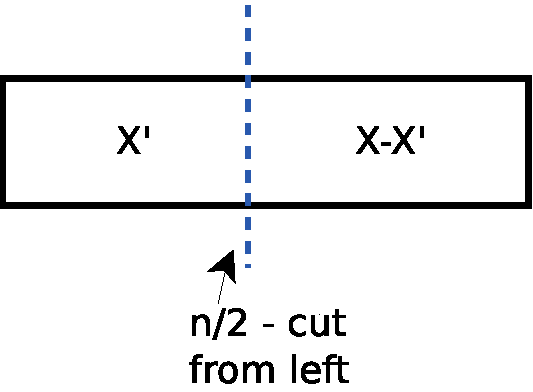
\includegraphics[width=180pt]{bilder/dc1.pdf}
   \caption{D$\&$C step 3}
  	 \end{figure}
\begin{lem}
The Divide-and-Conquer protocol is strategyproof for proportional protocols.
\end{lem}
\begin{proof} 
\textcolor{white}{x}\\\\
The proof can be found in \cite{dc}: We showed in section 2 that D$\&$C guarantees a player a proportional share 
if it is truthful.  We now consider the case when two players, $A$ and $B$, must divide a 
cake, but one may not be truthful.  If their truthful $\nicefrac{1}{2}$ points are as shown below, then 
cutting the cake at $|$ gives each player more than $\nicefrac{1}{2}$: 
$$0-----------a-|-b------------1$$ 
But if player $A$ should report that its $\nicefrac{1}{2}$ point is either to the left or right of a, it risks 
getting less than $\nicefrac{1}{2}$ the cake if $(i) |$ is to the left of a or $(ii) |$ is to the right of $b$.  This argument for the vulnerability of D$\&$C-that it does not guarantee a player a proportional 
share if it is not truthful-can readily be extended to $n > 2$ players.
\end{proof}
\begin{lem}
The Divide-and-Conquer protocol is game-theoretic strategyproof.
\end{lem}
\begin{proof}
\textcolor{white}{x}\\\\
\end{proof}
\newpage
%%%%%%%%%%%%%%%%%%%%%%%%%%%%%%%%%%%%%%%%%%%%%%%%%%%%%%%%%%%%%%%%%%%%%%%%%%%%%%%%%%%%%%%%%%%%%%%%%%%%%%%%%%%%%%%%
%%%%%%%%%%%%%%%%%%%%%%%%%%%%%%%%%%%%%%%%%%%%%%%%%%%%%%%%%%%%%%%%%%%%%%%%%%%%%%%%%%%%%%%%%%%%%%%%%%%%%%%%%%%%%%%%
%%%%%%%%%%%%%%%%%%%%%%%%%%%%%%%%%%%%%%%%%%%%%%%%%%%%%%%%%%%%%%%%%%%%%%%%%%%%%%%%%%%%%%%%%%%%%%%%%%%%%%%%%%%%%%%%
\section{Conclusion}
%In this work the common proportional cake-cutting protocols have been rewritten in a game-theoretic manner and analysed on whether a non-truthful strategy could yield a more advantageous situation for a non-truthful player. It was possible to approve game-theoretically that the only strategy which promises the best outcome is the strategy recommended by the protocol.\\
%The approach is very different from \cite{chen:truth} and \cite{tamuz}. In their approaches, the basic assumptions of cake-cutting is weakened and so only special cases are analysed. Instead the goal here was to adapt the existing definitions of truthfulness to the general cake-cutting problem.
\begin{table}[htb]
 \renewcommand{\arraystretch}{1.5} 
\begin{tabular*}{\textwidth}{|@{\extracolsep{\fill}}l|c|c|c|c|c|c|}
\hline
$\:$Protocol & \multicolumn{1}{c|}{WSP} & GTSP & GTCCSP & SP & SPP &SSP  \\
\hline
$\:$Cut $\&$ Choose & \Checkmark & \Checkmark  & \Checkmark &\Checkmark & \Checkmark &  \XSolidBrush\\
\hline
$\:$Last Diminisher & \Checkmark & \Checkmark & \Checkmark  &\Checkmark& \Checkmark &  \XSolidBrush\\
\hline
$\:$Lone Chooser & \Checkmark & \Checkmark & \Checkmark  &\Checkmark & \Checkmark &  \XSolidBrush\\
\hline
$\:$Lone Divider & \Checkmark & \XSolidBrush & \XSolidBrush & \XSolidBrush &\XSolidBrush & \XSolidBrush \\
%\hline
%$\:$Cut your Own Piece & SPP & SP & \XSolidBrush & \Checkmark &GTCCSP& GSP \\
\hline
$\:$Divide $\&$ Conquer & \Checkmark & \Checkmark & \Checkmark &\Checkmark &\Checkmark &  \XSolidBrush \\
\hline
\end{tabular*}
\caption{Overview: Strategyproofness of proportional cake-cutting protocols}\label{ov}
\end{table}	 
\pagebreak
%%%%%%%%%%%%%%%%%%%%%%%%%%%%%%%%%%%%%%%%%%%%%%%%%%%%%%%%%%%%%%%%%%%%%%%%%%%%%%%%%%%%%%%%%%%%%%%%%%%%%%%%%%%%%%%%
%%%%%%%%%%%%%%%%%%%%%%%%%%%%%%%%%%%%%%%%%%%%%%%%%%%%%%%%%%%%%%%%%%%%%%%%%%%%%%%%%%%%%%%%%%%%%%%%%%%%%%%%%%%%%%%%
%%%%%%%%%%%%%%%%%%%%%%%%%%%%%%%%%%%%%%%%%%%%%%%%%%%%%%%%%%%%%%%%%%%%%%%%%%%%%%%%%%%%%%%%%%%%%%%%%%%%%%%%%%%%%%%%
\section{Open Questions and Future Research}
%It would be interesting to take a closer look on the DGEF in the egalitarian point of view. Due to the fact that a protocol is only fair if every player gets his fair share, it seems to be intuitively more fair, if $n-1$ player envies one rather than one player envies all of the other players. The definition could be:\\
%MDGEF= minimal guaranteed degree of envy-freeness = $\min\limits_{i\in \mathbb{N}}\{\sum\limits_{j\in\mathbb{N},i \neq j} p_i \nVdash p_j\}$\\ Compare Brams, Jones and Klamler (2007) individual envy-relation.\\
%\newline
%For two main listed reasons the influence of cooperative game theory is kept short in this work. One of them is the statement of Nash himself from \cite{Nash: non-cooperative Games, 1950} where he proposed, that each cooperative game can be displayed as a non-cooperative game with cooperation in the set of valid strategies. \\
%\begin{bsp}
%\label{bsp2}
%(Cooperative Cake-Cutting)\\
%After the win of the election in Turingville the member of President Church coalition wants to divide successfully the power in the country. Some of the members are aware of being unsatisfied with the outcome and so cooperate mutually to change the allocation.
%\end{bsp}
%An interesting aspect would be groupstrategyproofness. Hereby, groups have public valuations for group members.\\
%\newline
%An other approach about strategyproofness could be a consecutively allocation of several cakes. Then the cake-cutting-game could be interpreted as a repeated game. 

\pagebreak

%%%%%%%%%%%%%%%%%%%%%%%%%%%%%%%%%%%%%%%%%%%%%%%%%%%%%%%%%%%%%%%%%%%%%%%%%%
%%%%%%%%%%%%%%%%%%%%%%%%%%%%%%% ENDE TEXTTEIL %%%%%%%%%%%%%%%%%%%%%%%%%%%%
%%%%%%%%%%%%%%%%%%%%%%%%%%%%%%%%%%%%%%%%%%%%%%%%%%%%%%%%%%%%%%%%%%%%%%%%%%

\clearpage
\bibliography{references.bib}
\bibliographystyle{alphadin}
\thispagestyle{empty}
%\vspace*{\fill}g
\pagestyle{plain}
\clearpage

\listoffigures

\listoftables
\thispagestyle{empty}
%\pagebreak
\pagestyle{plain}
%\printindex
\end{document}